% MAIN DOCUMENT FOR MASTER THESIS
\documentclass[twoside,english, a4paper, 11pt]{shared/fysbachelor}
\usepackage[top=1.5in, bottom=1.5in, left=1in, right=1in]{geometry}
\usepackage[backend=biber,style=numeric,sorting=none]{biblatex}
%\usepackage[utf8]{inputenc}
\usepackage{fontspec}
\addbibresource{bibliography/bachelor_thesis.bib}

\usepackage{afterpage}
\newcommand\blankpage{%
    \null
    \thispagestyle{empty}%
    \addtocounter{page}{-1}%
    \newpage}
% TITLE
\author{Davide Saccardo}
\title{{\scshape Insert Title}}
\date{July 2018} 

% LOAD PACKAGES 
\usepackage{listings}
\usepackage{xcolor}
\usepackage{amsmath}
\usepackage{amssymb}
\usepackage{lipsum}
% \usepackage[hidelinks]{hyperref}s
\usepackage{hyperref}
\usepackage{slashed}
\usepackage{simplewick}
\usepackage{sidecap} 
\usepackage[titletoc]{appendix}

\usepackage{algorithm}
\usepackage{algpseudocode}

\usepackage{etoolbox}

\usepackage[compat=1.1.0]{tikz-feynman}
\usepackage{multicol}

\patchcmd{\part}{\thispagestyle{plain}}{\thispagestyle{part}}{}{}

\definecolor{grey}{rgb}{0.98,0.98,0.98}
\definecolor{codeRed}{rgb}{0.5, 0.027, 0.02}

% Code parameters
\lstset{language=c++}
\lstset{basicstyle=\small}
\lstset{backgroundcolor=\color{white}}
\lstset{frame=single}
\lstset{stringstyle=\ttfamily}
\lstset{keywordstyle=\color{codeRed}\bfseries}
\lstset{commentstyle=\itshape\color{gray}}
\lstset{showspaces=false}
\lstset{showstringspaces=false}
\lstset{showtabs=false}
\lstset{breaklines}

\setlength{\parskip}{11pt}
\setlength{\parindent}{0mm}

\lstset{
language=Python,
basicstyle=\footnotesize
frame=single,
backgroundcolor=\color{grey}
}

\lstset{
language=Matlab,
basicstyle=\footnotesize,
frame=single,
backgroundcolor=\color{grey}
}

\lstset{
language=C++,
backgroundcolor=\color{grey}
}

\lstdefinelanguage{GLSL}
{
sensitive=true,
morekeywords=[1]{
attribute, const, uniform, varying,
layout, centroid, flat, smooth,
noperspective, break, continue, do,
for, while, switch, case, default, if,
else, in, out, inout, float, int, void,
bool, true, false, invariant, discard,
return, mat2, mat3, mat4, mat2x2, mat2x3,
mat2x4, mat3x2, mat3x3, mat3x4, mat4x2,
mat4x3, mat4x4, vec2, vec3, vec4, ivec2,
ivec3, ivec4, bvec2, bvec3, bvec4, uint,
uvec2, uvec3, uvec4, lowp, mediump, highp,
precision, sampler1D, sampler2D, sampler3D,
samplerCube, sampler1DShadow,
sampler2DShadow, samplerCubeShadow,
sampler1DArray, sampler2DArray,
sampler1DArrayShadow, sampler2DArrayShadow,
isampler1D, isampler2D, isampler3D,
isamplerCube, isampler1DArray,
isampler2DArray, usampler1D, usampler2D,
usampler3D, usamplerCube, usampler1DArray,
usampler2DArray, sampler2DRect,
sampler2DRectShadow, isampler2DRect,
usampler2DRect, samplerBuffer,
isamplerBuffer, usamplerBuffer, sampler2DMS,
isampler2DMS, usampler2DMS,
sampler2DMSArray, isampler2DMSArray,
usampler2DMSArray, struct},
morekeywords=[2]{
radians,degrees,sin,cos,tan,asin,acos,atan,
atan,sinh,cosh,tanh,asinh,acosh,atanh,pow,
exp,log,exp2,log2,sqrt,inversesqrt,abs,sign,
floor,trunc,round,roundEven,ceil,fract,mod,modf,
min,max,clamp,mix,step,smoothstep,isnan,isinf,
floatBitsToInt,floatBitsToUint,intBitsToFloat,
uintBitsToFloat,length,distance,dot,cross,
normalize,faceforward,reflect,refract,
matrixCompMult,outerProduct,transpose,
determinant,inverse,lessThan,lessThanEqual,
greaterThan,greaterThanEqual,equal,notEqual,
any,all,not,textureSize,texture,textureProj,
textureLod,textureOffset,texelFetch,
texelFetchOffset,textureProjOffset,
textureLodOffset,textureProjLod,
textureProjLodOffset,textureGrad,
textureGradOffset,textureProjGrad,
textureProjGradOffset,texture1D,texture1DProj,
texture1DProjLod,texture2D,texture2DProj,
texture2DLod,texture2DProjLod,texture3D,
texture3DProj,texture3DLod,texture3DProjLod,
textureCube,textureCubeLod,shadow1D,shadow2D,
shadow1DProj,shadow2DProj,shadow1DLod,
shadow2DLod,shadow1DProjLod,shadow2DProjLod,
dFdx,dFdy,fwidth,noise1,noise2,noise3,noise4,
EmitVertex,EndPrimitive},
morekeywords=[3]{
gl_VertexID,gl_InstanceID,gl_Position,
gl_PointSize,gl_ClipDistance,gl_PerVertex,
gl_Layer,gl_ClipVertex,gl_FragCoord,
gl_FrontFacing,gl_ClipDistance,gl_FragColor,
gl_FragData,gl_MaxDrawBuffers,gl_FragDepth,
gl_PointCoord,gl_PrimitiveID,
gl_MaxVertexAttribs,gl_MaxVertexUniformComponents,
gl_MaxVaryingFloats,gl_MaxVaryingComponents,
gl_MaxVertexOutputComponents,
gl_MaxGeometryInputComponents,
gl_MaxGeometryOutputComponents,
gl_MaxFragmentInputComponents,
gl_MaxVertexTextureImageUnits,
gl_MaxCombinedTextureImageUnits,
gl_MaxTextureImageUnits,
gl_MaxFragmentUniformComponents,
gl_MaxDrawBuffers,gl_MaxClipDistances,
gl_MaxGeometryTextureImageUnits,
gl_MaxGeometryOutputVertices,
gl_MaxGeometryOutputVertices,
gl_MaxGeometryTotalOutputComponents,
gl_MaxGeometryUniformComponents,
gl_MaxGeometryVaryingComponents,gl_DepthRange},
morecomment=[l]{//},
morecomment=[s]{/*}{*/},
morecomment=[l][keywordstyle4]{\#},
}

% ------------------------------------------------- COLOR BOX
 

% MAIN DOCUMENT BEGINNING
\begin{document}

% LOAD COMMANDS
% Equations
\newcommand{\beq}{\begin{equation}}
\newcommand{\eeq}{\end{equation}}
\newcommand{\bpsi}{\bar{\psi}}
\newcommand{\dslash}{\slashed{\partial}}
\newcommand{\Dslash}{\slashed{D}}
\newcommand{\Lagr}{\mathcal{L}}
\newcommand{\cpp}{\texttt{C++ }} 
\newcommand{\mpi}{\texttt{MPI }} 
\newcommand{\CIT}{{\color{red}(CITATION NEEDED)}}
\newcommand{\LINK}{{\color{red}(REFLINK NEEDED)}}
\newcommand{\NOTE}[1]{{\color{red} #1 }}
\newcommand{\FIGURE}[1]{{\color{red} FIG: #1 }}
\newcommand{\capt}[1]{\caption{\footnotesize{ #1 }}}
\newcommand{\D}{\mathcal{D}}
\newcommand{\Tr}{\mathrm{Tr}}
\newcommand{\fig}[4][1.0]{
    \begin{figure}[htp!]
        \begin{center}
            \includegraphics[scale=#1]{#2}
        \end{center}
        \capt{#3}
        \label{#4}
    \end{figure}
}
\newcommand{\bea}{\begin{align*}}
\newcommand{\eea}{\end{align*}}

\tikzset{->-/.style={decoration={
  markings,
  mark=at position #1 with {\arrow{>}}},postaction={decorate}}}
  \tikzset{-<-/.style={decoration={
  markings,
  mark=at position #1 with {\arrow{<}}},postaction={decorate}}}

  \tikzset{
    ncbar angle/.initial=90,
    ncbar/.style={
        to path=(\tikztostart)
        -- ($(\tikztostart)!#1!\pgfkeysvalueof{/tikz/ncbar angle}:(\tikztotarget)$)
        -- ($(\tikztotarget)!($(\tikztostart)!#1!\pgfkeysvalueof{/tikz/ncbar angle}:(\tikztotarget)$)!\pgfkeysvalueof{/tikz/ncbar angle}:(\tikztostart)$)
        -- (\tikztotarget)
    },
    ncbar/.default=0.5cm,
    }

\tikzset{square left brace/.style={ncbar=0.5cm}}
\tikzset{square right brace/.style={ncbar=-0.5cm}}

\tikzset{round left paren/.style={ncbar=0.5cm,out=120,in=-120}}
\tikzset{round right paren/.style={ncbar=0.5cm,out=60,in=-60}}


\newcommand{\tikzcuboidd}[4]{% width, height, depth, scale
\begin{tikzpicture}[scale=#4]
\foreach \x in {0,...,#1}
{   \draw (\x ,0  ,#3 ) -- (\x ,#2 ,#3 );
    \draw (\x ,#2 ,#3 ) -- (\x ,#2 ,0  );
}
\foreach \x in {0,...,#2}
{   \draw (#1 ,\x ,#3 ) -- (#1 ,\x ,0  );
    \draw (0  ,\x ,#3 ) -- (#1 ,\x ,#3 );
}
\foreach \x in {0,...,#3}
{   \draw (#1 ,0  ,\x ) -- (#1 ,#2 ,\x );
    \draw (0  ,#2 ,\x ) -- (#1 ,#2 ,\x );
}
\end{tikzpicture}
}

\newcommand{\tikzcube}[2]{% length, scale
\tikzcuboidd{#1}{#1}{#1}{#2}
}



\maketitle

%\begin{acknowledgements}
%		\input{preface/acknowledgements}
%\end{acknowledgements}

\begin{dedication}
	\null\vfill
	\begin{flushright}
		
		\vspace{12pt}
	\end{flushright}
	\null\vfill
\end{dedication}

\clearpage
\cleardoublepage

% ABSTRACT AND ACKNOWLEDGMENTS
\begin{abstract}
	The concept of a thinking machine has always teased the human mind. In the last years, with the development of Machine Learning (ML) and Neural Networks (NN), the topic has become something more than a simple suggestion. Certainly, the  predictions of the possible applications of such technologies have helped to increase the enthusiasm towards it. In this context it is possible to mention the possibility of discovering new drugs or automating certain tasks.
Research as well as private companies have started to invest an increasing amount of money and time in order to develop the theoretical and applicative aspects of ML. This has led to the launch of many applications which deal with computer vision, speech as well as objects recognition, etc. In recent times, applications were found also in physics, economy, bionformatics and marketing.


We implement the concept of ML with NN to non-interacting bosons in an elliptical harmonic trap, a system used to simulate the behaviour of a Bose-Einstein condensate. The energy is computed through Variational Monte Carlo methods, where the trial wave-function is represented by the Gaussian-Binary Restricted Boltzmann Machine (RBM). Two sampling methods are discussed: Brute-Force Metropolis and Importance Sampling Metropolis-Hastings. The variational parameters are updated with the Stochastic Gradient Descent method. The errors are computed through the Blocking method which takes into account correlations between data. An outline of the algorithms as well as of the general structure of the code is provided. 

%In the process of developing the code, we benchmarked it in two cases. 
To benchmark our code, we consider two cases: non-interacting bosons in a spherical harmonic trap and non-interacting bosons in an elliptical (along the z direction) harmonic trap. In the first one, the results agree with the previsions with good precision. In the second case, the results are not compatible with the analytical ones: the RBM seems to be ineffective in learning the elliptical symmetry. The problem is fixed by biasing the RBM's parameters which involve the z-ax. Then, we apply the code to the case of interacting (through hard-core potential) bosons in an elliptical harmonic trap. The data obtained are compared to the results furnished by the Gross-Pitaevskii (GP) equation in \cite{DalfString}. Even though, in some cases, our data underestimate the GP's one, the overall trend seems to be compatible. The final result $E_L/N_p=\SI{2.63\pm 0.02}{}\ \hbar \omega_{ho}$ with $N_p=100$ is found to agree well with the GP prediction.
 
 

%0.05 learning rates for NH>=4 in elliptical
	\clearpage
\end{abstract}


\tableofcontents
\clearpage 

\begin{chapter}{Introduction}
	\label{chap:intro}
	  In recent times Machine Learning (ML) methods using Neural Networks (NN) have become increasingly better at simulating quantum systems. In \cite{carleoSolvingQuantumManybody2017} Carleo and Troyer discuss the impressive potential of ML and NN methods over traditional methods.  In their article, they apply the so-called Binary-Binary Restricted Boltzmann Machine (RBM) to the quantum mechanical spin lattice systems of the Ising model and Heisenberg model, with
encouraging results. \\
In general, the topic of Machine Learning and Neural Network is gaining a lot of success: people are using such algorithms in different contexts such as speech (e.g. Google Translate) or objects (e.g. plants, handwritten numbers, etc.) recognition. Such applications are interesting, but they are not that important for physics. Nowadays research is more focused on using ML to understand which are the most important (biased) paths connecting, for example, two states (configurations). Usually each path would be considered, but this could lead to an impossible problem to deal with. However, by knowing which paths are more important, with a good approximation, it could be possible to exclude the least important ones. As a consequence, the problem is simplified. Examples could be provided by excited states in nuclear physics (carried out by coupled-cluster methods) or lattice QCD.

In this thesis we will test the applicability of the RBM to the Bose-Einstein condensate (BEC) to compute its ground state energy. The ground state energy of a BEC is a well known result \cite{DalfString}. Therefore our aim is not to introduce something new in that direction but to check whether the ML approach could be used also here and whether we can learn something more about ML itself. The basic idea is to use a NN of visible and hidden nodes to represent a system wave-function $\Psi$. The weights of these nodes act as variational parameters leading to the convenient use of the variational method to approximate the ground state. The energy of $\Psi$ is calculated and the (Stochastic) Gradient Descent (SGD) method is applied to find the set of parameters that minimize the energy function. In particular we use a Gaussian-Binary RBM as choice of NN to represent $\Psi$.

First of all, we study one and two non-interacting bosons in a 1D, 2D and 3D spherical harmonic potential. We consider such a small number of particles just for the sake of computational speed. Anyway, this case is particularly useful: the system becomes a harmonic oscillator and thus we have analytical solutions that we can use to benchmark our code. Then, we study the same system in a 3D elliptical harmonic potential. We look for possible changes in the system due to the different potential's symmetry adopted. Finally we study the case of interacting bosons in a 3D elliptical harmonic potential. We skip the 2D case since for the three dimensional one we have results to benchmark ours. The interaction between bosons is modeled with a hard-core potential.

The ground state energy is computed through Variational Monte Carlo (VMC) methods, a class of iterative technique employing the repeated use of random sampling and statistical analysis to solve mathematical problems. The goal is to reproduce a probability distribution through the generation of samples. As they are produced, their values follow more and more precisely the desired distribution. At each interaction, the program chooses a candidate from the class of samples based on the current sample (even though improperly, we could also say that the program makes a choice). Then, this candidate is either accepted or rejected with a certain probability. Two aspects are particularly important (strongly connected with each other): the first is how samples are generated (i.e. a sampling rule) and the second is the so-called accept-reject rule. The computational algorithms which describe the accept-reject rule are the Metropolis algorithms. Hence, when a choice of the sampling rule is made, a choice of the accept-reject rule follows and thus a choice of the Metropolis algorithm used. In this paper, we consider two possibilities: a Brute-Force way of generating a sample which leads to the so-called Metropolis algorithm (in the following, we will refer to this procedure as Brute-Force Metropolis algorithm, BFM) and the Importance Sampling way of generating samples which leads to the Metropolis-Hastings algorithm for accepting-rejecting moves (in the following, Importance-Sampling Metropolis-Hastings algorithm, ISMH). In BFM the sampling rule is independent on the trial wave-function and thus it is not really efficient. ISMH is a much better alternative since it proposes moves biased by the trial wave-function that are more likely to be accepted.  Overall the system becomes much better at reproducing the probability distribution.\\
%The basic difference between a normal VMC calculation and our code is related to the trial wave-function as well as to the variation of the variaitonal parameter. 

The results are presented with an appropriate statistical error computed through blocking method which takes into account correlations between data.

The code is object oriented in order to achieve the best flexibility possible. In principle it should be straightforward to (let us say) change the initial configurations of particles, to study systems of fermions or to change the potential.

\section{Bose-Einstein condensate}
A Bose-Einstein condensate is a state of matter in which dilute gases of bosons undergo a phase transition when they are cooled to low temperature ($T\rightarrow 0\ \si{\kelvin}$). As a result the majority of bosons condense into the system ground state (Bose-Einstein condensation, BEC). This gives rise to new quantum phenomena such as superfluidity and phase coherence \cite{Stringari}. 

The concept was proposed for the first time by A. Einstein in 1925 who followed the work of the Indian physicist S. N. Bose (1924) on the statistics of photons and applied it to a gas of non-interacting, massive bosons. However the prediction remained without any practical meaning until the 1938, when F. London realized that BEC could be responsible for the superfluidity in $^4$He. Since the interaction between  atoms in helium is strong \cite{pethick_smith_2008}, it is difficult to measure effectively the number of particles in the condensate. Therefore, research focused on weakly-interacting Bose gases with a higher condensate fraction such as alkali atoms. They were eventually achieved in 1995 by the teams of Cornell and Wieman at Boulder with $^{87}$Rb and of Ketterle at MIT with $^{23}$Na cooled down to temperature of the order of $100\ \si{\nano\kelvin}$ through laser cooling and evaporative cooling in magneto-optical traps. For this discovery, they shared the Nobel prize in 2001. 

%Bose–EinsteinCondensationinDiluteGases C. J. Pethick Nordita H. Smith University of Copenhage

%dalfovo article
Since these experiments involve the use of traps, the gases are naturally nonuniform. Moreover, as said above, gases are considered to be dilute which means that the average distance between atoms is much larger than the range of the inter-atomic interaction. Therefore the reference equation is the Gross-Pitaevskii (GP) equation:
\beq
\label{GP}
i\hbar\frac{\partial \Psi (\mathbf{r},t)}{\partial t}=\bigg(-\frac{\hbar^2}{2m}\nabla^2+V(\mathbf{r})+g|\Psi(\mathbf{r},t)|^2\bigg)\Psi(\mathbf{r},t)
\eeq
%\CIT %stringar
where $i=\sqrt{-1}, \hbar$ is the reduced Planck constant, $t$ is time, $\Psi$ is the condensate wave-function, $\mathbf{r}$ represents the position of bosons and $V$ is the external potential which confines the bosons. The quantity $g$ is the coupling constant 
\begin{equation*}
	g=\frac{4\pi\hbar^2a}{m}
\end{equation*}
where $a$ is the s-wave scattering length. GP equation describes inhomogeneous dilute gases such as alkali atoms in magneto-optics trap, its solution will be used to benchmark our results.

In this paper, we compute the ground-state energy of the Bose-Einstein gas and we compare the results with the ones found in literature \cite{DalfString}, where the approach used was steepest descent to minimize the energy functional which describes the ground-state energy in the Gross-Pitaevskii framework. There the physics is dominated by two-body collisions and it can be described through s-wave scattering length $a$. The condition of diluteness is given by the parameter $na^3$, where $n$ is the density of the system. When low values of this parameter are considered the Gross-Pitaevskii theory works very well. However, in some experiments the parameter may exceed the such values. In these cases it may be important to study the problem with a many-body approach. In literature many papers are found of Monte Carlo calculations where a broad range of densities is studied by going beyond the GP equation. For example, in \cite{vmcarticle}, Dubois and Glyde use Variational Monte Carlo (VMC) methods to study the Bose gas from dilute to liquid $^4$He densities. Basically the same range is considered by Giorgini et al. in \cite{Giorgini}, where, conversely, the Diffusion Monte Carlo (DMC) approach is performed, and in Gr\"{u}ter et al. \cite{Gruter}, where the path-integral Monte Carlo is chosen. \\
In this thesis, we use ML and we compare the results with GP equation since we consider a diluite system. Nevertheless, out of the diluite range, we note that ML results should be compared to the Monte Carlo ones which we have briefly mentioned above. 


%Monte Carlo methods with their several variants (diffusion VMC, coupled-cluster, etc) have been use extensively since their development by Ulam in the $1940s-1950s$ to study many-body problem. Our first procedure is basically the quantum mechanics' variational method applied through a Monte Carlo evaluation with a given trial wave-function (\CIT). The variational method allows us to find the an upper limit to the ground state energy which depends on a variational parameter. Therefore the variational parameter $\alpha$ which minimizes the energy is the one that will give the best estimate for the ground state. The gradient descent method is applied to find the optimal $\alpha$. %for both interacting and non case. The non-interacting case is used to prove the efficiency of the method since the best variational parameter can be easily computed.



%In both situations 
 

%\section{Structure of the Thesis}
%\cref{part:intro}
%The Thesis is organized in three sections. In the first one the general system is discussed. Then 
\end{chapter}

%% PART I: INTRODUCTORY STUFF
%\begin{part}{Overview of Bose-Einstein condensations}
%	\label{part:intro}
%
%	% \begin{chapter}{Discretization Effects in Lattice Yang-Mills Theories and Scale Fixing}
%	% 	\label{chap:problem_intro}
%	%   	\input{introduction/problem_intro}
%	% \end{chapter} 
%\end{part}


% PART II: IMPLEMENTATION
\begin{part}{Implementation}
	\label{part:implementation}
	
	\begin{chapter}{The system}
		\label{chap:system}
		We consider a gas of $N_p$ bosons in spherical and elliptical harmonic oscillator potentials. The interaction between bosons is modeled by the hard-core model as in \cite{vmcarticle}. %We set $\hbar = m = 1$. 
The Hamiltonian of the system is 
\begin{equation}
H = \sum_{i=1}^{N_p}\left[ -\frac{1}{2}\frac{\hbar^2}{m}\nabla_i^2 + V_{ext}(\textbf{r}_i) \right]+ \sum_{i \neq k} V_{int}(r_{ik}),
\label{eq_hamilton}
\end{equation}
where $V_{ext}(\textbf{r})$ is the harmonic oscillator potential given by
\begin{equation*}
V_{ext}(\textbf{r})=\begin{cases}
\frac{1}{2}m\omega_{ho}^2r^2 &\text{Spherical}\\
\frac{1}{2}m\left[ \omega_{ho}^2 \left(x^2 + y^2 \right) + \omega_z^2 z^2\right] &\text{Elliptical}
\end{cases}
\end{equation*}
and $V_{int}(r_{ik})$ is the hard-core interaction potential 
\begin{equation*}
V_{int}(r_{ik}) = \begin{cases}
 0, & r_{ik} > a \\
 \infty, & r_{ik} < a.
\end{cases}
\end{equation*}
The quantity $r_{ik} = |\textbf{r}_i-\textbf{r}_k|$ represents the distance between particle $i$ and $k$, while $a$ is the size of the interaction between particles. 

\paragraph{No interaction - spherical trap} When we set the interaction to be zero ($V_{int}=0$), we are left with a harmonic oscillator potential, where we consider a spherical shape for simplicity. In this case the solutions are known analytically. In general the energy is given by $E_n=\hbar\omega_{ho}(n+\frac{1}{2})$. The ground state is 
\begin{equation*}
E(N_p,\text{D}) = \frac{1}{2}\text{D} N_p\ \hbar\omega_{ho}.
\label{analitica}
\end{equation*}
where D is the dimension of the system and $N_p$ is the number of particles. This case is useful to benchmark our code at the beginning.

\subparagraph{No interaction - elliptical trap}
The interaction is still null ($V_{int}=0$), the trap now is considered to be elliptical.\\
Let us introduce lengths in unit of $a_{ho}=\sqrt{\hbar/(m\omega_{ho)}}$, $r\rightarrow r/a_{ho}$ and energy in units of $\hbar\omega_{ho}$. The Hamiltonian can be rearranged as 
\begin{equation*}
\begin{split}
H&=\sum_{k=1}^{N_p}\bigg(-\frac{\hbar^2}{2m}\nabla^2_{k}+\frac{1}{2}m[\omega^{2}_{ho}(x^2_k+y^2_k)+\omega^{2}_{z}z_k^2]\bigg)\\
&=\sum_{k=1}^{N_p}\frac{\hbar \omega_{ho}}{2}\bigg(-\frac{\hbar}{m\omega_{ho}}\nabla^2_{k}+\frac{\omega_{ho}m}{\hbar}\bigg[x^2_k+y^2_k+\frac{\omega^{2}_{z}}{\omega^{2}_{ho}}z^2_k\bigg]\bigg)\\
&=\sum_{k=1}^{N_p}\frac{\hbar \omega_{ho}}{2}\bigg(-a_{ho}\nabla^2_{k}+a_{ho}{\hbar}\bigg[x^2_k+y^2_k+\frac{\omega^{2}_{z}}{\omega^{2}_{ho}}z^2_k\bigg]\bigg).
\end{split}.
\end{equation*}
We set $\lambda=\omega_z/\omega_{ho}$, we get
\begin{equation}
\label{ham}
H=\sum_{k=1}^{N_p}\frac{1}{2}\bigg(-\nabla^2_{k}+V_{ext}(\mathbf{r}_k)\bigg)
\end{equation}
where $V_{ext}=x^2_k+y^2_k+\lambda^2 z^2_k$. As in \cite{DalfString}, we set $\lambda=\sqrt{8}$. In \cite{vmcarticle}, the energy of non-interacting bosons in this trap is shown to be

\begin{equation*}
	\frac{E}{N}\rightarrow E_{ho}=\hbar\omega_{ho}\bigg(1+\frac{\lambda}{2}\bigg)=2.414\ \hbar\omega_{ho}.
\end{equation*}

We will use this result to benchmark again our code.

\subparagraph{Interaction - elliptical trap}
At this point, we turn on the interaction $V_{int}\neq 0$ and we consider an elliptical trap. The Hamiltonian is

\begin{equation}
\label{ham2}
H=\sum_{k=1}^{N_p}\frac{1}{2}\bigg(-\nabla^2_{k}+V_{ext}(\mathbf{r}_k)\bigg)+\sum_{k<i}^{N_p} V_{int}(\mathbf{r}_k,\mathbf{r}_i).
\end{equation}
where $V_{ext}=x^2_k+y^2_k+\lambda^2 z^2_k$ and $\lambda=\sqrt{8}$ as above.
%\noindent During the whole project, we will use natural units $\hbar=m=\omega_{ho}=1$.

\section{Methods}
To compute the ground state energy of bosons, we use the variational method from quantum mechanics which gives an upper bound for the ground state energy $E_{gs}$ given a trial wave-function $\Psi_T$: 
\begin{equation}
\label{var_princ}
E_{gs}\leq \frac{\braket{\Psi_T|H|\Psi_T}}{\braket{\Psi_T|\Psi_T}}\boldsymbol=\frac{\int \Psi_T^{*}(\textbf{X},\boldsymbol{\theta})H\Psi_T(\textbf{X},\mathbf{\theta})d\textbf{X}}{\int \Psi_T^{*}(\textbf{X},\boldsymbol{\theta})\Psi_T(\textbf{X},\boldsymbol{\theta})d\textbf{X}}.
\end{equation}
In eq. (\ref{var_princ}), $\mathbf{X}$ represents the particles' positions and $\boldsymbol{\theta}$ represent the variational parameters. With Machine Learning, the variational parameters are the biases of the NN. Hence $\boldsymbol{\theta} = a_1, \dots, a_\text{N},  b_1, \dots, b_\text{M}, w_{11}, \dots, w_{\text{NM}}$. The quantities N and M are respectively the number of visible and the number of hidden nodes. \\
The integral in eq. (\ref{var_princ}) is impossible to evaluate with methods such as Gaussian quadrature in a reasonable amount of time. In such a situation, Monte Carlo methods are needed.

Let us consider a trial wave-function and define the probability density function (PDF) 
\begin{equation}
\label{PDF}
P(\mathbf{X},\boldsymbol{\theta})=\frac{|\Psi_T|^2}{\int d\textbf{X}|\Psi_T|^2}
\end{equation}
and define the local energy as
\begin{equation}
\label{local_energy}
E_L=\frac{1}{\Psi_T}H\Psi_T.
\end{equation}
By using eq. (\ref{PDF}) and eq. (\ref{local_energy}), we have
\begin{equation*}
E_{gs}\leq  \frac{\int d\mathbf{X} \Psi^{*}_{T}H\Psi_T}{\int d\mathbf{X}|\Psi_T|^2}=\int d\mathbf{X}\  P(\mathbf{X},\boldsymbol{\theta})E_L(\mathbf{X},\boldsymbol{\theta})\simeq \frac{1}{N_{MC}}\sum_{i=1}^{N}P(\mathbf{X}_i,\boldsymbol{\theta})E_L(\mathbf{X}_i,\boldsymbol{\theta})
\end{equation*}
where $N_{MC}$ is the number of Monte Carlo steps.

%With the basic VMC method, our variational parameter is represented by a value which we call $\alpha$. Therefore to find the minimum energy we can use MC methods to compute the mean local energy for different alphas and then see which alphas return the minimum energy. An automated version of this is to use numeric methods that finds function minimums based on the calculations from the MC cycles. For instance conjugate gradient and gradient descent are good iterative methods. We will implement the gradient descent method: the outline is to do some MC cycles to calculate quantities needed for the numeric minimum finder per iteration, eventually the numeric method will find a minimum and return an optimal $\alpha$. Then we can do MC sampling with many more steps on the system with the optimal parameters. This is a proper variational Monte Carlo \cite{morten_book} (VMC) method. 

We will use MC methods to calculate the local energy for a set of Gaussian distributed $\boldsymbol{\theta}$, then we will apply the Stochastic Gradient Method (SGD) (more in section \ref{sec_SGD}) to find a new $\boldsymbol{\theta}$ that will give a lower energy. This is an iterative method to find a function minimum. The final result should be a good estimate for the ground state. Since the SGD method has to be applied many times, the number of MC cycles for each SGD iteration should not be very large (to save time). Rather once the SGD cycles have finished we do a run of the final set of parameters with a large number of MC cycles to give a final answer.

However this method will not always be applicable. If the RBM is not able to converge to a precise energy but notably fluctuates, then it is not meaningful to use a final set of variational parameters for a final MC run. Instead the SGD local energy is used. We average the SGD data after equilibration. This will produce a mean local energy that can be used as a final result.

\subsection{Sampling methods}
We use MC methods to measure system quantities such as energy by generating samples that reproduce more and more precisely the desired distribution. The basic recipe is to choose one particle randomly, and propose in a certain way a step for that particle. Then according to a certain rule either accept or decline the move. We will use two methods to propose and accept/reject moves: Brute-Force Metropolis (BFM) and Importance Sampling Metropolis-Hastings (ISMH) \cite{morten_book}. 

\subsubsection{Brute-Force Metropolis algorithm}
The standard Metropolis algorithm (also referred to as Brute-Force Metropolis in this text) follows the basic recipe (referred to as a "brute-force" sampling rule) for choosing new positions given by
\begin{equation*}
x_{k+1} = x_k + Lr,
\end{equation*}
where $L$ is a step length and $r$ is a uniformly distributed random variable $\in [0,1]$. We accept moves that are deemed likely by the ratio of the absolute square wave-functions before and after the move. We choose a new random number r, and if
\begin{equation}
r \leq \frac{|\Psi_T(\textbf{r}_{k+1})|^2}{|\Psi_T(\textbf{r}_{k})|^2},
\label{eq_accept_move}
\end{equation}
then we accept the move. If it is not verified, we decline it. 

\subsubsection{Importance Sampling Metropolis-Hastings algorithm}
The issue with BFM is that the algorithm proposes a lot of moves that get rejected. The independence of the sampling rule with respect to the trial wave-function is responsible for this behaviour. These rejected moves cause a lot are wasted computation time and as such, it becomes desirable to use an algorithm that proposes moves that are more likely to be accepted. In order to obtain this, we will use the Importance Sampling way of generating samples.

The basic idea behind Importance Sampling is to propose moves corresponding to an isotropic diffusion
process with a drift. Such a process obeys Fokker-Planck equation 
\begin{equation*}
\frac{\partial P}{\partial t} = D\frac{\partial}{\partial x}\left(\frac{\partial}{\partial x}-F\right)P,
\end{equation*}
where $P$ is the probability density function of the system, $D$ is the diffusion coefficient and $F$ is the drift force. This equation governs the time evolution of the probability density function for a diffusing system under random forces. In the bosonic system the probability density function is the wave-function itself and we call $F$ the quantum force. The diffusion coefficient assumes the value $1/2$ ($D = 1/2$) due to the half factor in the kinetic energy. 

The solution of the Fokker-Planck equation is 
\begin{equation*}
F = \frac{2\nabla \Psi_T}{\Psi_T}.
\end{equation*}
and the new move is given by the following sampling rule
\begin{equation*}
x_{k+1} = x_k + DF\Delta t + r\sqrt{\Delta t},
\end{equation*}
where $\Delta t$ is some time step parameter that can be tuned. 

Now that we have changed the sampling rule we need to alter the method of accepting/rejecting such moves. We move then to the Metropolis-Hastings algorithm. The probability of diffusion can be solved from the Fokker-Planck equation through a Green function
\begin{equation*}
G(x_{k+1},x_k,\Delta t) = \frac{1}{(2\pi\Delta t)^{3N/2}}\exp\left[ -\frac{\left(x_{k+1} - x_{k} - \Delta tF(x_k)\right)^2}{2\Delta t}  \right].
\end{equation*}
The new moves are now accepted following the rule 
\begin{equation}
r \leq \frac{G(x_k, x_{k+1}, \Delta t)|\Psi_T(x_{k+1})|^2}{G(x_{k+1}, x_{k}, \Delta t)|\Psi_T(x_{k})|^2},
\label{eq_imp_sam}
\end{equation}
where $r$ is a Gaussian distributed random number. 

\subsection{Iterative methods to find optimal variational parameters}
In order to obtain the minimum energy, we need to adjust the variational parameters $\boldsymbol{\theta}$.% for the ML case.
Therefore we introduce the Stochastic Gradient Descent (SGD) method.

%\subsubsection{Gradient descent}
%Sometimes referred to as steepest descent, the gradient descent method is an iterative method used to find local minima of functions. The basic idea is to choose an initial $\textbf{x}$ and find a new $\textbf{x}$ following
%\begin{equation*}
%\textbf{x}_{k+1} = \textbf{x}_{k} - \lambda_k \nabla f(\textbf{x}_k),
%\end{equation*}
%where $\lambda_n$ is some factor, preferably small. If the derivative is negative, then $x$ will increase. If the derivative is positive, $x$ will decrease. At the minimum the derivative will be zero and thus the method will converge. There are many gradient descent methods which differ by choice of $\lambda_n$. The ideal method is to have some algorithm such that $\lambda$ approaches zero when the function approaches the minimum. This project will use constant $\lambda$. The simple algorithm can be implemented as
%\begin{lstlisting}
%while (iter < maxIterations && energyDerivative < tolerance){	
%x -= lambda*gradF(x)
%}	
%\end{lstlisting} 
%An issue with the gradient descent method is that it can only find local minimum without knowing whether it is the global one or not. This can be bypassed by running the algorithm multiple times with different initial guesses. If they converge to the same minimum, it is a good indication that the function only has one local(global) minimum. 

\subsubsection{Stochastic Gradient Descent (SGD)} \label{sec_SGD}
The method of choice used to optimize our RBM is the Stochastic Gradient Descent. The basic idea is that we want to find the minimum of the local energy as a function of the variational parameters $\boldsymbol{\theta}$. This is done by following the direction of the negative gradient towards the minimum. The set of parameters is $\boldsymbol{\theta} = (a_1...a_\text{N},b_1,...b_\text{M},w_{11},w_{\text{NM}})$. The method updates the parameters by 
\begin{align}
	\label{parameter}
\boldsymbol{\theta}_{k+1} = \boldsymbol{\theta}_k - \eta \nabla E_L(\boldsymbol{\theta}),
\end{align}
where $\eta$ is the learning rate of our RGB. We use a fixed learning rate. There are methods that use adaptive $\eta$ to speed up or optimize minimum searches. One potential downside to this method is that it is impossible to know whether the method has found a local minimum or the global minimum. In this project it is the global minimum we are interested in.

We can find expressions for the gradient of the local energy with respect to the parameters. The general expression is
\begin{equation}
\frac{\partial\langle E_{L}\rangle}{\partial \boldsymbol{\theta}_k} = 2 \left[ \langle \frac{E_{L}}{\Psi}   \frac{\partial\Psi}{\partial\boldsymbol{\theta}_k} \rangle - \langle E_{L} \rangle \langle \frac{1}{\Psi}\frac{\partial\Psi}{\partial\boldsymbol{\theta}_k} \rangle  \right].
\label{eq_energy_gradient}
\end{equation}
To compute this value, the derivatives with respect to the parameters of the wave-function are needed. These can be solved analytically with straightforward methods. For simplicity we define $s_k = \exp(-b_k-\sum_i^M\frac{X_iW_{ik}}{\sigma^2})$. The derivatives are then found as
\begin{equation*}
\frac{1}{\Psi}\frac{\partial\Psi}{\partial a_k} = \frac{X_k-a_k}{\sigma^2}
\label{eq_grad_ak}
\end{equation*}
\begin{equation*}
\frac{1}{\Psi}\frac{\partial\Psi}{\partial b_k} = \frac{1}{1 + s_k}
\label{eq_grad_bk}
\end{equation*}
\begin{equation*}
\frac{1}{\Psi}\frac{\partial \Psi}{\partial w_{kl}} = \frac{X_k}{\sigma^2} \frac{1}{1+s_l}
\label{eq_grad_wk}
\end{equation*}
Then, the program has to sample these quantities during the MC steps to create the means required in Eq. (\ref{eq_energy_gradient}).

\subsection{Statistical analysis - blocking method}
It is important to have an estimate for the error of our results. The simple way of getting an error estimate is to take the standard deviation of our data. The issue with that method is that the standard deviation does not take the correlation of the data into account and, in this thesis, in fact, data are correlated. It is simple to see that because the energy is a time series: the energy does change discontinuously, in Monte Carlo steps, but the change is typically small compared to the total energy and thus it can be classified as a time series.

An excellent tool for analyzing time series correlation is the blocking method \cite{marius}. The basic idea is to start with a correlated dataset and turn it into an uncorrelated dataset which we take the standard deviation of. The method works in this way: suppose that our initial dataset is 
\begin{equation*}
\textbf{X}_0 = (X_1,X_2,...,X_N)\quad \text{where}\ X_1=(\mathbf{X_0})_1,
\end{equation*}
we average $X_1$and $X_2$ and place it into $(\textbf{X}_1)_1$. Then we do the same for $X_3$ and $X_4$ and place it in $(\textbf{X}_1)_2$ and so on. This is one blocking iteration. Our new array is less correlated because the elements are further from each other than in the original time series.

By following the calculations of \cite{marius}, the variance of the data set after blocking $k$ times is
\begin{equation*}
V(\bar{\textbf{X}}_k) = \frac{\sigma^2_k}{n_k} + \frac{2}{n_k}\sum_{h=1}^{n_k-1}\left(  1-\frac{h}{n_k} \right)\gamma_k(h) = \frac{\sigma^2_k}{n_k} + \epsilon_k ,
\end{equation*}
where $\bar{\textbf{X}}_k$ is the mean of $\textbf{X}_k$, $\sigma_k$ is the standard deviation in $\textbf{X}_k$, $n_k$ is the number of elements in $\textbf{X}_k$ and $\gamma_k$ is the autocovariance of $\textbf{X}_k$. We call $\epsilon_k$ the truncation error. It can be shown \cite{marius} that $\epsilon_k$ tends to zero as we keep on blocking. The result is that the error of the mean is just the standard deviation of the data set. This error should better reflect the error of our results than the simple standard deviation and it should also be larger since it takes into account correlations.

The blocking method is specifically useful for large data sets since the computation cost is of the order of $O(n)$ whereas other methods are $O(n^2)$ or worse. Indeed, when we are dealing with data sets sizes of the order of $10^6 - 10^7$, there is a large speed difference between $O(n)$ and $O(n^2)$. 

\subsection{Structure of the code}
The code is written in C++, object-oriented in order to allow small changes (such as a different choice of potential) without notching the overall code. The general structure of the algorithm is the following:
  
\begin{lstlisting}
- generate parameters throught Gaussian distribution with sigma=0.5 or 0.1 or 0.01

for(int cycles = 0; cycles < TotalNumberOfCycles; cycles ++){ //SGD cycle
	
	- Compute trial wave-function and quantum force
	
	for (int i = 0; i < numberOfMetropolisSteps; i++) {  //Monte Carlo cycle
	
		- Brute-Force Metropolis or Importance Sampling Metropolis-Hastings
		- Sample the quantities we are interesting in such as energy
	
	}
	
	- Compute averages: average energy
	- Stochastic Gradient Descent: change parameters and use them for the next cycle
}
\end{lstlisting} 

The data are analyzed through python scripts, where the Blocking method is adopted and plots are made. The codes can be found in \url{https://github.com/DavideSaccardo/BEC_ML_thesis}.

\section{Trial Wave-function}
In this section we show the trial wave-function chosen % for the basic VMC case and the one chosen for the ML case. 
and we compute interesting quantities (such as local energy, quantum force). 

\subsection{ML trial wave-function}
We choose to represent our trial wave-function with a set of artificial Neural Networks. We call this way of representing the trial wave-function, Neural-Network Quantum State (NQS) \cite{carleoSolvingQuantumManybody2017}. In particular, the architecture selected is the Restricted Boltzmann Machine. It consists of one layer of visible nodes and one layer of hidden nodes. Each node represents a neuron-like unit where calculations take place: in our case the visible nodes represent the positions of bosons. The nodes are connected to each other across layers, but nodes of the same layer are not linked in the "restricted" machine. In the unrestricted one, connections between hidden nodes are allowed. Therefore there is a connection from every node in the visible layer to every node in the hidden layer (see Fig. (\ref{Fig:draw}) for a representation). 

In general, the goal of the RBM is to learn the probability distribution of the simulated system. In quantum systems the probability distribution is the wave-function $\Psi$. The outputs we wish to produce are the positions of the bosons.  

\begin{figure}
	\centering
	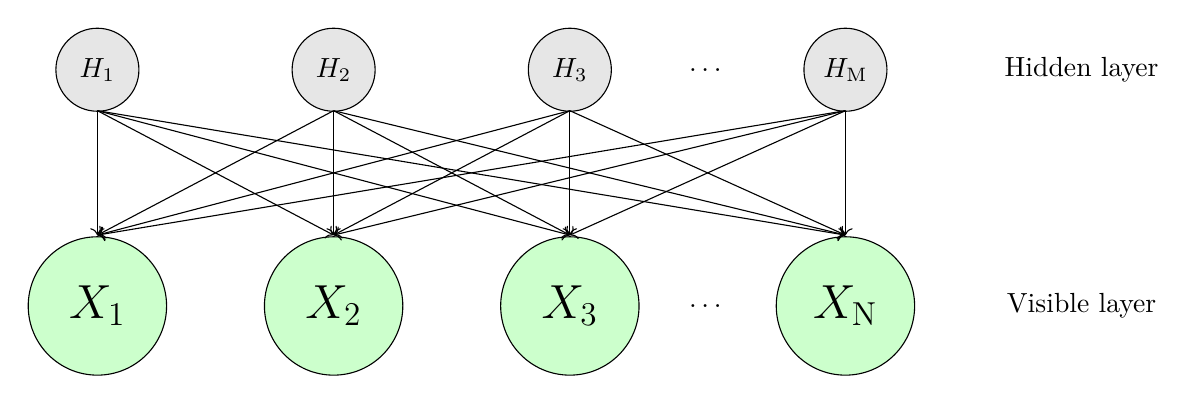
\begin{tikzpicture}
	\draw[black,fill=gray,fill opacity=0.2] (-4.5,0) circle (15pt) node[text=black, fill opacity=1] {$H_1$};
	\draw[black,fill=gray,fill opacity=0.2] (-1.5,0) circle (15pt) node[text=black, fill opacity=1] {$H_2$};
	\draw[black,fill=gray,fill opacity=0.2] (1.5,0) circle (15pt) node[text=black, fill opacity=1] {$H_3$};
	\node[draw, white, text=black] at (3.25,0) {$\dots$};
	\node[draw, white, text=black] at (8,0) {Hidden layer};
	\node[draw, white, text=black] at (8.0,-3) {Visible layer};
	\draw[black,fill=gray,fill opacity=0.2] (5,0) circle (15pt) node[text=black, fill opacity=1] {$H_\text{M}$};
	\draw[black,fill=green,fill opacity=0.2] (-4.5,-3) circle (25pt) node[text=black, fill opacity=1, align= center] {\LARGE $X_1$};
	\draw[black,fill=green,fill opacity=0.2] (-1.5,-3) circle (25pt) node[text=black, fill opacity=1] {\LARGE$X_2$};
	\draw[black,fill=green,fill opacity=0.2] (1.5,-3) circle (25pt) node[text=black, fill opacity=1] {\LARGE$X_3$};
	\node[draw, white, text=black] at (3.25,-3) {$\dots$};
	\draw[black,fill=green,fill opacity=0.2] (5,-3) circle (25pt) node[text=black, fill opacity=1] {\LARGE$X_\text{N}$};
	\draw[black,->] (-4.5,-0.52) to (-1.5,-2.1);
	\draw[black,->] (-4.5,-0.52) to (-4.5,-2.1);
	\draw[black,->] (-4.5,-0.52) to (1.5,-2.1);
	\draw[black,->] (-4.5,-0.52) to (5,-2.1);
	\draw[black,->] (-1.5,-0.52) to (-1.5,-2.1);
	\draw[black,->] (-1.5,-0.52) to (-4.5,-2.1);
	\draw[black,->] (-1.5,-0.52) to (1.5,-2.1);
	\draw[black,->] (-1.5,-0.52) to (5,-2.1);
	\draw[black,->] (1.5,-0.52) to (-1.5,-2.1);
	\draw[black,->] (1.5,-0.52) to (-4.5,-2.1);
	\draw[black,->] (1.5,-0.52) to (1.5,-2.1);
	\draw[black,->] (1.5,-0.52) to (5,-2.1);
	\draw[black,->] (5,-0.52) to (-1.5,-2.1);
	\draw[black,->] (5,-0.52) to (-4.5,-2.1);
	\draw[black,->] (5,-0.52) to (1.5,-2.1);
	\draw[black,->] (5,-0.52) to (5,-2.1);
	\end{tikzpicture}
	\caption{Sketch of a Neural Network Quantum State: it shows the architecture of a Restricted Boltzmann Machine applied to our quantum many-body problem. The visible layer ($X_i$, with $i=1,\dots,$N) is a set of N visible neurons which take as input the positions of the particles, whereas the hidden layer ($H_j$, with $j=1,\dots,$M) is a set of M invisible neurons.}
	\label{Fig:draw}
\end{figure}


The joint probability distribution of the RBM is defined as 
\begin{equation*}
F_{RBM}(\textbf{X},\textbf{H}) = \frac{1}{Z} \exp(-E(\textbf{X},\textbf{H})),
\end{equation*}
where \textbf{X} is the visible nodes and \textbf{H} is the hidden nodes. The quantity $Z$ represents the partition function or normalization constant of the system. 

The quantity $E(\textbf{X},\textbf{H})$ is the function that specifies the relation between the visible and hidden nodes. It is called the energy of the node configuration. This is different from the energy of the quantum mechanical system. The choice of $E(\textbf{X},\textbf{H})$ defines the kind RBM we have. In the bosonic case, the visible nodes need to take continuous values to properly represent the particle positions. We then look at the Gaussian-Binary RBM. In other cases it might be more desirable to have binary outputs (as Carleo and Troyer used for the Ising Model in \cite{carleoSolvingQuantumManybody2017}). For those cases the Binary-Binary RBM can be used. The Gaussian-Binary RBM is given as 
\begin{equation*}
E(\textbf{X},\textbf{H}) = \sum_i^{\text{N}}\frac{(X_i-a_i)^2}{2\sigma} - \sum_j^{\text{M}}b_jH_j + \sum_{ij}^{\text{N,M}}\frac{X_iw_{ij}H_j}{\sigma^2},
\label{eq_rbm}
\end{equation*}
where \textbf{a} is the visible bias, \textbf{b} is the hidden bias and $\textbf{w}_{ij}$ is the weight of the connection between visible node $i$ and hidden node $j$. We have N visible nodes and M hidden nodes. To represent the particle positions, N has to be the number of particles $\times$ the number of dimensions.  The general recipe is to take fewer hidden nodes than the visible ones.

To represent the wave-function, we use the so-called "marginal PDF" found by summing over all the hidden nodes:
\begin{equation*}
\Psi(\textbf{X}) = \sum_HF_{RBM}(\textbf{X},\textbf{H}) = \frac{1}{Z}\sum_H\exp(-E(\textbf{X},\textbf{H})).
\end{equation*}
Setting in the Gaussian-Binary RBM gives the final result
\begin{equation*}
\Psi(\mathbf{X}) = \frac{1}{Z} \exp\bigg[-\sum_i^{\text{N}} \frac{(X_i-a_i)^2}{2\sigma^2}\bigg]\prod_j^{\text{M}} \left(  1 + \exp\bigg[b_j +\sum_i^{\text{N}} \frac{X_iw_{ij}}{\sigma^2}\bigg]\right).
\label{eq_psi}
\end{equation*}
As stated above, the aim of the RBM is to learn a probability. To accomplish this task, the bias $\mathbf{a},\mathbf{b}$ and the weights $\mathbf{w_{ij}}$ need to be modified according to a rule, which in our case is to minimize the energy. We will obtain that some connections between nodes are more weighted than others: in fact, this is the utility of Machine Learning i.e. to understand which connections are more favored than others, this skill could be important in some cases to reduce significantly problems that are impossible to deal with at the beginning.

\subsubsection{Analysis of Hamiltonian}
The local energy is defined as 
\begin{equation*}
E_L = \frac{1}{\Psi(\textbf{X})}\textbf{H}\Psi(\textbf{X}) = \frac{1}{\Psi(\textbf{X})} \left(\sum_{k=1}^{N_p} -\frac{1}{2}\nabla_k^2 + V_{ext}(\mathbf{r}_k)\right)\Psi(\textbf{X})+\sum_{k<i}^{N_p} V_{int}(\mathbf{r}_k,\mathbf{r}_i).
\label{eq_loc_e}
\end{equation*}
Now let us focus on the term $\nabla^2\Psi$. It can be solved analytically. We start by taking the gradient, the derivative is with respect to the visible nodes. We look at the gradient with respect to the coordinates of the $j$'th particle. We begin with using the product rule:
\begin{align*}
\nabla_j\Psi(\textbf{X}) = -\left(\sum_{k=j}^{j+\text{D}}\frac{X_k-a_k}{\sigma^2}\hat{\textbf{X}}_k \right) e^{\sum_i^{\text{N}}\frac{(X_i-a_i)^2}{2\sigma^2}} \prod_l^{\text{M}}\left(1+e^{b_L}e^{\sum_i^{\text{N}}\frac{X_iW_{il}}{\sigma^2}}\right) \\
+ e^{\sum_i^{\text{N}}\frac{(X_i-a_i)^2}{2\sigma^2}} \sum_ {i=j}^{j+\text{D}}\prod_{l\neq j}^{\text{M}} \left(1+e^{b_l}e^{\sum_i^{\text{N}}\frac{X_iW_{il}}{\sigma^2}}\right) e^{b_j}e^{\sum_i^{\text{N}}\frac{X_iW_{il}}{\sigma^2}}\sum_ {k=j}^{j+\text{D}}\frac{W_{kl}}{\sigma^2}\hat{\textbf{X}}_k,
\end{align*}
where $\hat{\textbf{X}}_k$ is the unit vector in the direction of $\textbf{X}_k$ and D is the number of dimensions. We can collect terms and recognize $\Psi(\textbf{X})$ in the expression above. We have
\begin{equation}
\nabla_j \Psi(\textbf{X}) = \Psi(\textbf{X})\left(  -\sum_{k=j}^{j+\text{D}} \frac{X_k-a_k}{\sigma^2} \hat{\textbf{X}}_k  + \sum_{l}^{\text{M}}\frac{e^{b_l}e^{\sum_{i}^{\text{N}}\frac{X_iW_{il}}{\sigma^2}}}{1+e^{b_l}e^{\sum_{i}^{\text{N}}\frac{X_iW_{il}}{\sigma^2}}}  \sum_{k=j}^{j+\text{D}} \frac{W_{kl}}{\sigma^2} \hat{\textbf{X}}_k    \right).
\label{eq_gradient}
\end{equation}
When finding the laplacian it will be convenient to treat the gradient as one expression. Using the product rule we then get
\begin{align*}	
\nabla^2_j \Psi(\textbf{X}) = \frac{(\nabla_j \Psi(\textbf{X}) )^2}{\Psi(\textbf{X})} + \Psi(\textbf{X})\left[ \sum_{k=j}^{j+\text{D}}-\frac{1}{\sigma^2} + \sum_{l=1}^{\text{M}} \frac{e^{b_l}e^{\sum_{i}^{\text{N}}\frac{X_iW_{il}}{\sigma^2}}\sum_{k=j}^{j+\text{D}} \frac{W_{kl}^2}{\sigma^4}  \Big(1+e^{b_l}e^{\sum_{i}^{\text{N}}\frac{X_iW_{il}}{\sigma^2}}\Big)}{\Big(1+e^{b_l}e^{\sum_{i}^{\text{N}}\frac{X_iW_{il}}{\sigma^2}}\Big)^2} \right.  \\ \left. - \frac{ e^{b_l}e^{\sum_{i}^{\text{N}}\frac{X_iW_{il}}{\sigma^2}}\sum_{k=j}^{j+\text{D}} \frac{W_{kl}}{\sigma^2} \hat{\textbf{X}}_k e^{b_l}e^{\sum_{i}^{\text{N}}\frac{X_iW_{il}}{\sigma^2}} }{\Big(1+e^{b_l}e^{\sum_{i}^{\text{N}}\frac{X_iW_{il}}{\sigma^2}}\Big)^2}   \sum_{k=j}^{j+\text{D}} \frac{W_{kl}}{\sigma^2} \hat{\textbf{X}}_k     \right]  \\
= \frac{(\nabla_j \Psi(\textbf{X}) )^2}{\Psi(\textbf{X})} + \Psi(\textbf{X})\left[-\frac{\text{D}}{\sigma^2} + \sum_{l=1}^{\text{M}}  \frac{e^{b_l}e^{\sum_{i}^{\text{N}}\frac{X_iW_{il}}{\sigma^2}}  \Big(1+e^{b_l}e^{\sum_{i}^{\text{N}}\frac{X_iW_{il}}{\sigma^2}}\Big) - e^{b_l}e^{\sum_{i}^{\text{N}}\frac{X_iW_{il}}{\sigma^2}}}{\Big(1+e^{b_l}e^{\sum_{i}^{\text{N}}\frac{X_iW_{il}}{\sigma^2}}\Big)^2}  \sum_{k=j}^{j+\text{D}} \frac{W^2_{kl}}{\sigma^4}      \right]\\
= \frac{(\nabla_j \Psi(\textbf{X}) )^2}{\Psi(\textbf{X})} + \Psi(\textbf{X})\left[ -\frac{\text{D}}{\sigma^2} + \sum_{l=1}^{\text{M}}   \frac{e^{b_l}e^{\sum_{i}^{\text{N}}}\frac{X_iW_{il}}{\sigma^2}  }{\Big(1+e^{b_l}e^{\sum_{i}^{\text{N}}\frac{X_iW_{il}}{\sigma^2}}\Big)^2}  \sum_{k=j}^{j+\text{D}} \frac{W^2_{kl}}{\sigma^4}      \right]
\end{align*}
Finally we wish to look at the laplacian normalized by the wave-function. The result is 
\begin{equation*}
\frac{\nabla_j^2\Psi(\textbf{X})}{\Psi(\textbf{X})}= \left(\frac{\nabla_j \Psi(\textbf{X}) }{\Psi(\textbf{X})}\right)^2 - \frac{\text{D}}{\sigma^2}  + \sum_{l=1}^{\text{M}}   \frac{e^{b_l}e^{\sum_{i}^{\text{N}}}\frac{X_iW_{il}}{\sigma^2}  }{\Big(1+e^{b_l}e^{\sum_{i}^{\text{N}}\frac{X_iW_{il}}{\sigma^2}}\Big)^2}  \sum_{k=j}^{j+\text{D}} \frac{W^2_{kl}}{\sigma^4}     
\label{eq_laplace}
\end{equation*}


\paragraph{Quantum force}
The gradient is already calculated in Eq. (\ref{eq_gradient}). Dividing by $\Psi(\textbf{X})$ we get the quantum force 
\begin{equation*}
\textbf{F}_j = \frac{2\nabla\Psi}{\Psi}=  2\left(  -\sum_{k=j}^{j+\text{D}} \frac{X_k-a_k}{\sigma^2} \hat{\textbf{X}}_k  + \sum_{l}^{\text{M}}\frac{e^{b_l}e^{\sum_{i}^{\text{N}}\frac{X_iW_{il}}{\sigma^2}}}{1+e^{b_l}e^{\sum_{i}^{\text{N}}\frac{X_iW_{il}}{\sigma^2}}}  \sum_{k=j}^{j+\text{D}} \frac{W_{kl}}{\sigma^2} \hat{\textbf{X}}_k    \right).
\label{eq_quantumforce}
\end{equation*}


	\end{chapter}
	
%	\begin{chapter}{Variational Monte-Carlo}
%  		\label{chap:VMC}
%  		\input{implementation/VMC}
%	\end{chapter}
%
%	\begin{chapter}{Machine Learning}
%		\label{chap:ML}
%		\input{implementation/ML}
%  \end{chapter}
\end{part}


% PART III: RESULTS
\begin{part}{Data Analysis and Results}
	\label{part:results}
	\begin{chapter}{Non-interacting bosons in a spherical and elliptical harmonic trap}
	Before presenting the results for the interacting bosons in an elliptical trap, we study the non-interacting system with the spherical and elliptical trap. This is important to benchmark our code in order to understand that is working appropriately. At the beginning we concentrate on understanding how the system reacts in the spherical trap by tuning parameters such as BFM step length, ISMH time step, and learning rate. Eventually the energies from the different sampling methods are presented together. Then, we consider the same system in an elliptical trap. 
We note that all the standard deviations $\sigma$ presented hereafter are calculated through Blocking method: the correlations between data are taken into account. 

\section{Non-interacting bosons in a spherical harmonic trap}

In the non-interacting case, the best solution is when the $\boldsymbol{b}$ and $\boldsymbol{w}$ are close to zero. Therefore, if we choose a small standard deviation when generating initial  parameters, we will already start with a guess that is close to the final solution. This is not very interesting, because it does not allow us to see the RBM's developments. Therefore we set the parameter $\sigma=0.5$ to give a spread and an initial energy that is not correct. In this way we can clearly see how the RBM adapts to the desired distribution. We consider just one and two particles in 1D, 2D and 3D. We choose such a small number of particles for computational speed reasons. We study the system with both Brute-Force Metropolis and Importance Sampling Metropolis-Hastings algorithms to understand which one performs better.

\subsection{BFM algorithm}
First of all, we study how the system reacts when the step length of the BFM is changed. In Fig. (\ref{Fig:1}), we show how the SGD energy optimizes towards equilibrium for various BFM step lengths with a learning rate $\eta=0.01$ applied to 2 particles in 2 dimensions and 2 hidden nodes. In this case, from eq. (\ref{analitica}), we expect the correct energy to be $E_L=2\ \hbar\omega_{ho}$. 

\begin{figure}[H]
\centering
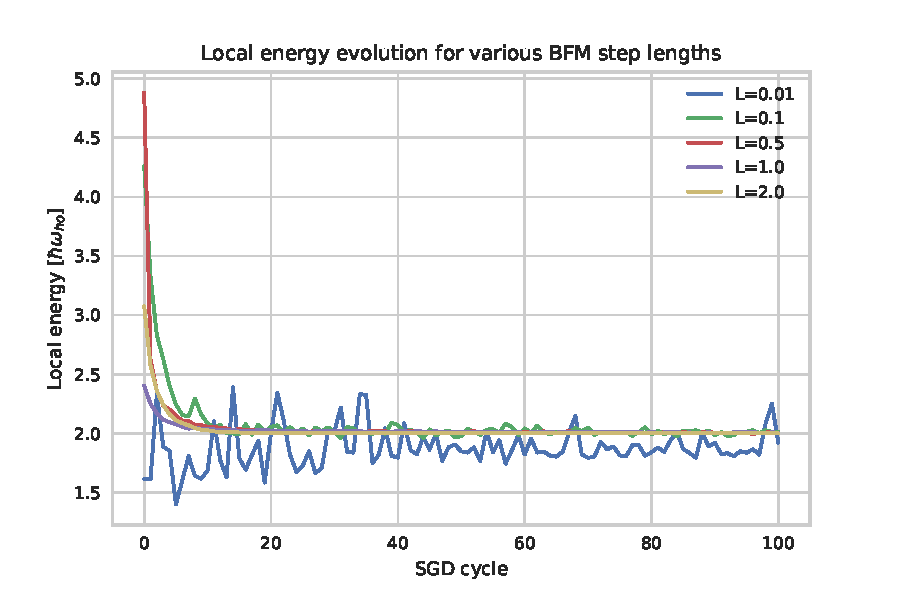
\includegraphics[scale=1.0]{plot1.pdf}
\caption{Local energy evolution calculated as the program adapts using Stochastic Gradient Descent for various Metropolis step lengths. Two particles in two dimensions with two hidden nodes and $\eta = 0.1$ are considered. We note how for $L\geq 0.5$ are quite stable at $E_L=2\ \hbar\omega_{ho}$.}
\label{Fig:1}
\end{figure}

As we can see from the figure, $L=0.01$ underestimates the correct value and the system does not equilibrate, $L=0.1$ oscillates around the correct value for a long time. On the other hand for $L\geq0.5$ equilibrium is reached after only a few cycles, which is desirable. Therefore it appears that a larger step length produces a faster equilibrium. This is reasonable: with a large step length particles are more moved at each step and thus even though we start with a bad configuration, we will reach faster a good one through the SGD. It appears that $L=1.0$ is the fastest one to converge. 
Moreover we study also the behaviour of the acceptance ratio of Monte Carlo steps as a function of the step length. The results are shown in Tab. (\ref{Tab:1}). We note that using a very large $L$ results in a small acceptance ratio and by consequence we sample the same positions many times, effectively producing worse statistics. Therefore it is desirable to use a step length that results in a higher acceptance ratio. 

\begin{table}[H]
\caption{Acceptance ratio as function of BFM step length. The data are made using  2 particles in 2 dimensions with 2 hidden nodes.}
\centering
\begin{tabular}{c| c } 
\textbf{L} & \textbf{Acceptance ratio} \\ \hline
2.0  & 0.73   \\
1.0 & 0.85  \\
0.5  &  0.93 \\
0.1  &  0.985 \\
0.01  &  0.999 \\ 
\end{tabular}
\label{Tab:1}
\end{table} 

%Each SGD cycle notes the standard deviation of the local energy. 
In Fig. (\ref{Fig:2}) we study the evolution of the standard deviation computed through the blocking method (which takes into account correlations of data) of the local energy as the the SGD cycles advance. From the figure we can extract that by using small step length ($L=0.01,0.1$) the error is larger than the other cases and that the standard deviation undergoes large fluctuations. On the other hand for larger step length, the fluctuations as well as the errors decrease.

\begin{figure}[H]
	\centering
	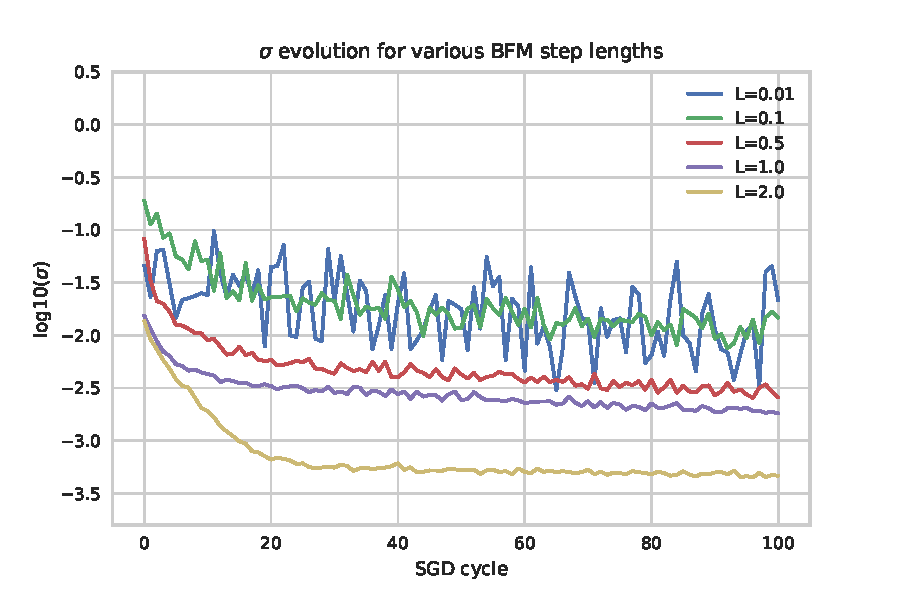
\includegraphics[scale=1.00]{plot2.pdf}
	\caption{Local energy evolution calculated as the program adapts using Stochastic Gradient Descent for various BFM step lengths. Two particles in two dimensions with two hidden nodes and $\eta = 0.1$ are considered. As we increase the BFM step length, the value of $\sigma$ as well as its fluctuation decrease with the exception of the first two step length.}
	\label{Fig:2}
\end{figure} 

By combining the data from Fig. (\ref{Fig:1}), Fig. (\ref{Fig:2}) and Tab. \ref{Tab:1}, we conclude that $L = 1.0$ is an appropriate choice of step length for the BFM algorithm. Also $L=0.5,2.0$ could be good choices, but $L=1.0$ is the most balanced one: it has a good acceptance ratio, low $\sigma$ and it is the fastest to converge.

To understand how the learning works and which is the best learning rate to use, we plot in Fig. (\ref{Fig:3}) the SGD energy optimization of the RBM applied to 2 bosons in 2D for multiple learning rates. The figure shows that small learning rates use a long time to converge. Learning rate $\eta=0.01$ does converge to the same value after approximately 100 SGD cycles, $\eta=0.05$ converges after 50 cycles and the others converge with less than 10 cycles. We verify that increasing $\eta$ beyond 0.6 results in a diverging energy. 

\begin{figure}[H]
\centering
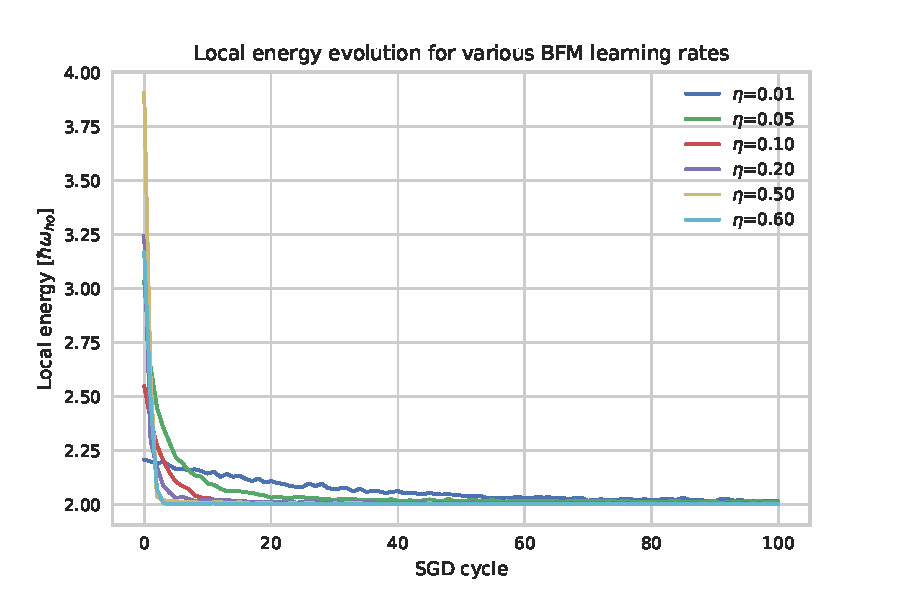
\includegraphics[scale=1.00]{plot3.pdf}
\caption{Local energy evolution calculated with BFM algorithm as the program adapts using SGD for two particles in 2D. BFM step length 1.0 is used for all the runs. Smaller learning rates give slower convergence.}
\label{Fig:3}
\end{figure}


\subsection{ISMH algorithm}

As we have done above with the BFM, we study the system with the Importance Sampling Metropolis-Hastings algorithm by taking into account its behaviour as we change the time step $\Delta t$. 

In Fig. (\ref{Fig:4}) the SGD cycle energy adaption for multiple ISMH $\Delta t$  is shown. The data are made using $\eta = 0.1$. We can see that the velocity of convergence for $\Delta$ t $\in [0.001,2.00]$ is almost the same. However, in the case of $\Delta t=0.001$, the system does not converge well to the energy minimum: this is the only data series that visibly fluctuates. From this we can conclude that we should use $\Delta t > 0.001$. 

\begin{figure}[ht]
\centering
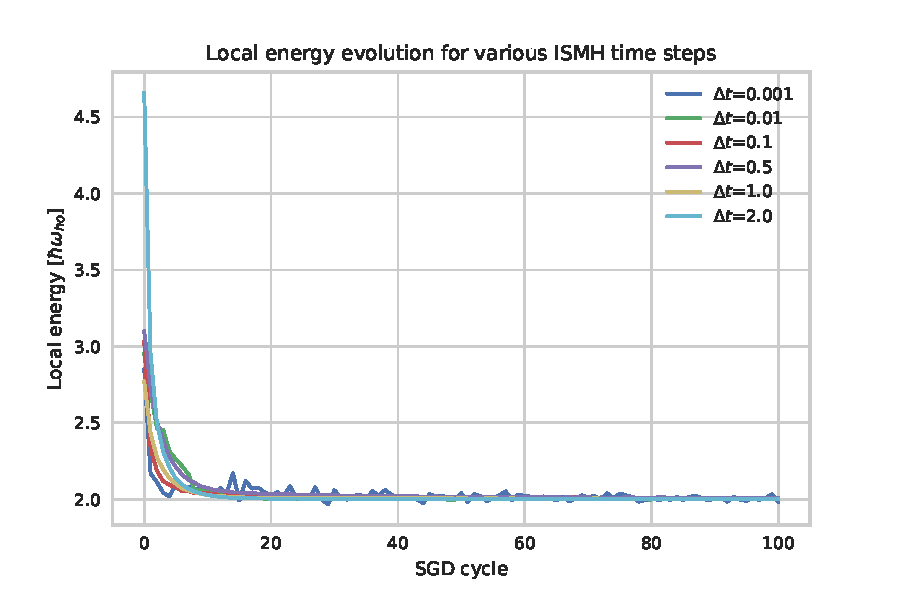
\includegraphics[scale=1.0]{plot4.pdf}
\caption{Local energy evolution calculated with ISMH algorithm as the program adapts using SGD for two particles in 2D. The data are made using $\eta = 0.1$ and 2 hidden nodes. The convergence time is very fast, and is almost independent of $\Delta t$. By using $\Delta t=0.5$ the process is faster than with the other time steps. All the time steps converge to the same energy. By using $\Delta t = 0.001$, the local energy fluctuates visibly for 100 cycles. It will therefore be favorable to use $\Delta t > 0.001$.}
\label{Fig:4}
\end{figure}
At this point we plot (Fig. (\ref{Fig:5})) the logarithm of the standard deviation of the local energy of the data from Fig. (\ref{Fig:4}) as function of SGD cycles. The data show that by increasing the time step the $\sigma$ decreases even though for $\Delta t\in [1.0, 2.0]$ is almost the same. Moreover the standard deviation becomes smoother as the time step increases. 

\begin{figure}[H]
\centering
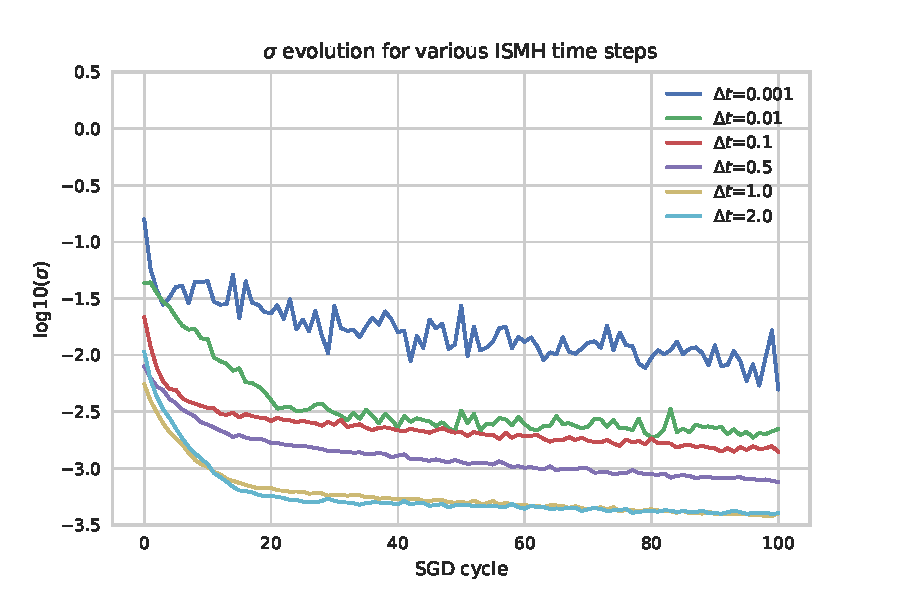
\includegraphics[scale=1.0]{plot5.pdf}
\caption{Logarithm of the standard deviation evolution calculated with ISMH algorithm as the program adapts using SGD for two particles in 2D. The data are made using $\eta = 0.1$. $\Delta t\leq 0.05$ use a long time to converge to the energy. It will therefore be favorable to use $\Delta t > 0.05$.}
\label{Fig:5}
\end{figure}
% 1.3.2 learn rate 0.1
In Tab. \ref{Tab:2}, we show the acceptance rate of Monte Carlo steps using ISMH as a function of $\Delta t$. Again we wish to have a large acceptance ratio. This ratio should not be close to one, though.  In fact that would mean that we are accepting all the moves which is a signal that we are not moving enough the particles at each Monte Carlo step. From the table, the best option is obviously $\Delta t = 0.5$. 

\begin{table}[H]
\centering
\caption{Acceptance ratio as function of ISMH time step. The data are made using 2 particles in 2 dimensions and 2 hidden nodes.}
\begin{tabular}{c| c } 
\textbf{$\boldsymbol{\Delta}$t} & \textbf{Acceptance ratio} \\ \hline
2 & 0.49 \\
1 & 0.78 \\
0.5 & 0.92  \\
0.1  &  0.993 \\
0.05  &  0.997 \\
0.01  &  0.9998 \\
0.001 & 0.99999 \\ 
\end{tabular}
\label{Tab:2}
\end{table} 

By combining this with the considerations expressed above, we conclude $\Delta t= 0.5$ is an acceptable time step, it will be used in the further computations. 

When it comes to the learning rate, we note that varying $\eta$ (Fig. (\ref{Fig:6})) produces results similar to the ones of Fig. (\ref{Fig:3}): $\eta=0.01$ converges really slowly in about more than 100 cycles, whereas the other learning rates converges almost with the same speed.



\begin{figure}[H]
\centering
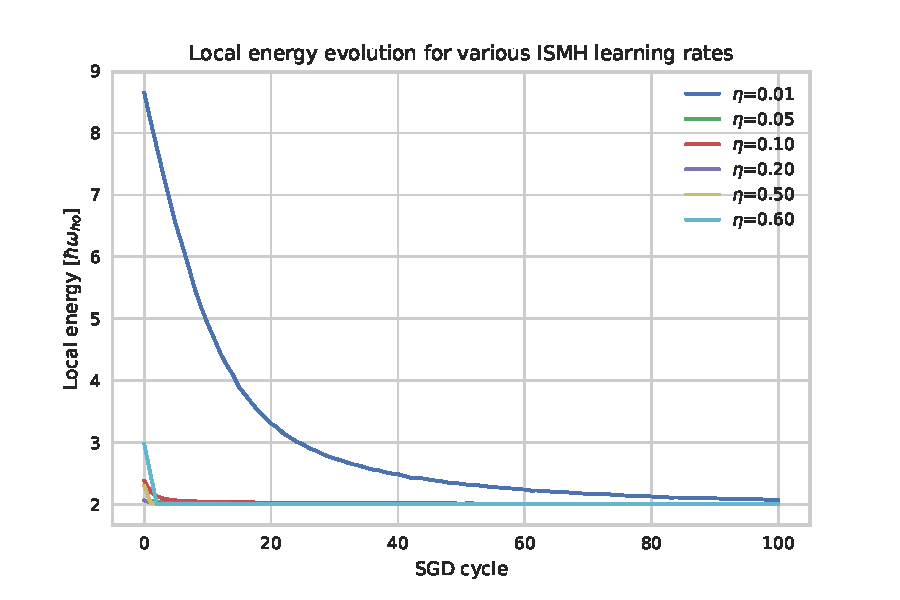
\includegraphics[scale=1.0]{plot6.pdf}
\caption{Local energy evolution calculated with ISMH algorithm sampling as the program adapts using SGD for two particles in 2D. Importance Sampling time step 0.5 is used for all the runs. Even though all the learning rates converge, we note that $\eta=0.01$ converges really slowly.}
\label{Fig:6}
\end{figure} 


\subsection{Energy of non-interacting bosons in a spherical harmonic trap}
Having found all the "right" parameters for each sampler, we proceed to give some values of energy for different configurations of particles, dimensions and number of hidden nodes. We use as learning rate $\eta=0.6$ because it seems the largest stable and we want the fastest convergence. After some running, we have understood that by increasing the number of hidden nodes and with D $=3$, the system gets more instable and thus we have to decrease the learning rate: we set $\eta=0.2$ when M $=4$ and $\eta=0.1$  when D $=3$.

In Tab. \ref{Tab:3}, we show the ground state local energy of non-interacting bosons computed with the different samplers. Results regarding one and two particle in 1D and 2D agree really well with the analytical predictions. On the other hand, the agreement between the analytical results and the samplers data in 3D is not good. This might suggest that we should have used more cycles for the convergence. In general it appears ISMH produces smaller errors than BFM. For both algorithms the error increases as more hidden nodes are added.  

\begin{table}[H]
\centering
\caption{Local energy of non-interacting bosons in a spherical harmonic trap. The quantity $N_p$ is the number of bosons, D is the dimensionality, M is the number of hidden nodes and $\eta$ is the learning rate. We show the analytical results and the ones obtained with BFM as well as ISMH algorithms. The setup consists on 300 SGD cycles of 300 000 MC steps. The final run to compute the energy is done with $10^7$ MC steps. The BFM step length is $L=1.0$, ISMH time step is $\Delta t = 0.5$. Both algorithms use $\sigma = 1.00$.  The error is calculated using the blocking method.}
\begin{tabular}{c c c c |c c c} 
$\boldsymbol{N_p}$ & \textbf{D}  & $\boldsymbol{M}$ & $\eta$ & \textbf{Analytical} & \textbf{BFM} & \textbf{ISMH} \\
&&&&$[\hbar\omega_{ho}]$ &$[\hbar\omega_{ho}]$&$[\hbar\omega_{ho}]$\\\hline
1 & 1 & 1 & 0.6 & 0.5  & $\SI{0.50002\pm 0.00001}{}  $ & $\SI{0.500001\pm 0.000001}{}$ \\ \hline
1 & 2 & 1 &0.6 & 1.0   & $\SI{1.00003\pm 0.00002}{} $ & $\SI{1.000000\pm 0.000003}{}$ \\
1 & 2 & 2 &0.6 & 1.0   & $\SI{1.00003\pm 0.00002}{} $ & $\SI{1.00004\pm 0.00001}{}$ \\ \hline
1 & 3 & 1 &0.1 & 1.5  &  $\SI{1.5003\pm 0.0001}{} $ &  $\SI{1.50033\pm 0.00003}{}$\\
1 & 3 & 2 &0.1 & 1.5   &  $\SI{1.5005\pm 0.0001}{} $ & $\SI{1.50069\pm 0.00003}{}$ \\
1 & 3 & 3 &0.1 & 1.5   &  $\SI{1.5005\pm 0.0001}{}$&   $\SI{1.50058\pm 0.00003}{}$\\ \hline
2 & 1 & 1 &0.6 & 1.0  & $\SI{1.00006\pm 0.00002}{} $ & $\SI{1.00003\pm 0.00001}{}$ \\ 
2 & 1 & 2 &0.6 & 1.0  & $\SI{1.00003\pm 0.00001}{}$ & $\SI{1.00004\pm 0.00001}{}$ \\ \hline
2 & 2 & 1 &0.6 & 2.0  & $\SI{2.00009\pm 0.00003}{}$ & $\SI{2.00006\pm 0.00001}{}$ \\
2 & 2 & 2 &0.6 & 2.0   & $\SI{2.0002\pm 0.0003}{}$ & $\SI{2.00010\pm 0.00001}{}$ \\
2 & 2 & 3 &0.6 & 2.0   & $\SI{2.0001\pm 0.0004}{}$ & $\SI{2.00008\pm 0.00001}{}$ \\
2 & 2 & 4 &0.2 & 2.0   & $\SI{2.0007\pm 0.0001}{}$ & $\SI{2.00068\pm 0.00004}{}$ \\ \hline 
2 & 3 & 1 &0.1 & 3.0   &   $\SI{3.0012\pm 0.0002}{}$&  $\SI{3.0010\pm 0.0001}{}$ \\
2 & 3 & 2 &0.1 & 3.0   &   $\SI{3.0017\pm 0.0002}{}$&  $$\SI{3.0020\pm 0.0001}{}$$ \\
2 & 3 & 3 &0.1 & 3.0   &  $\SI{3.0026\pm 0.0003}{}$&    $\SI{3.0018\pm 0.0001}{}$ \\
2 & 3 & 4 &0.1 & 3.0   &  $\SI{3.0024\pm 0.0003}{}$&   $\SI{3.0036\pm 0.0001}{}$ \\
2 & 3 & 5 &0.1 & 3.0  &  $\SI{3.0036\pm 0.0003}{}$  &  $\SI{3.0039\pm 0.0001}{}$  \\
2 & 3 & 6 &0.1 & 3.0   &  $\SI{3.0044\pm 0.0003}{}$   & $\SI{3.0051\pm 0.0001}{}$  \\ 
\end{tabular}
\label{Tab:3}
\end{table} 

\section{Non-interacting bosons in an elliptical harmonic trap}
At this point, we change the shape of the harmonic trap: we consider the Hamiltonian in eq. (\ref{ham}). There are no reasons to think that the parameters found in the previous sections (such as BFM step length, ISMH time step) should change. Hence we use the same ones. Only the 3D case is involved in the change of symmetry since we modify the z direction. Therefore we focus our analysis on the 3D case. Again we only consider cases of one or two particles for computational speed. Nevertheless we decide to use the Importance Sampling Metropolis-Hastings algorithm since it has proved to be the one which gives smaller errors.  In Tab. (\ref{Tab:3.2}), we show the results obtained with the elliptical harmonic trap. In \cite{vmcarticle}, Dubois and Glyde show $E/N=2.414\ \hbar\omega_{ho}$ for this trap. As we can see from the table, the results are not compatible with the predictions for many standard deviations. This is unexpected. 

\begin{table}[H]
	\centering
	\caption{Local energy per particle $E_L/N_p$ of non-interacting bosons in an elliptical harmonic trap. The quantity $N_p$ is the number of bosons, D is the dimensionality, M is the number of hidden nodes and $\eta$ is the learning rate. We show the analytical results and the ones obtained with ISMH algorithm. The setup consists on 300 SGD cycles of 300 000 MC steps. The final run to compute the energy is done with $10^7$ MC steps. The ISMH time step is $\Delta t = 0.5$ and $\sigma = 1.00$.  The error is calculated using the blocking method.}
	\begin{tabular}{c c c c |c  c} 
		$\boldsymbol{N_p}$ & \textbf{D}  & $\boldsymbol{M}$ & $\eta$ & \textbf{Analytical} &\textbf{ISMH} \\
		&&&&$[\hbar\omega_{ho}]$ &$[\hbar\omega_{ho}]$\\\hline
		1 & 3 & 1 &0.1 &           2.414                &          $\SI{3.247\pm 0.002}{}$              \\
		1 & 3 & 2 &0.1 &           2.414                 &       $\SI{3.250\pm 0.002}{}$                 \\
		1 & 3 & 3 &0.1 &           2.414                 &       $\SI{3.251\pm 0.002}{}$                 \\ \hline
		2 & 3 & 1 &0.1 &           2.414                 &      $\SI{3.25\pm 0.01}{}$                  \\
		2 & 3 & 2 &0.1 &           2.414                 &      $\SI{3.25\pm 0.01}{}$                  \\
		2 & 3 & 3 &0.1 &           2.414                 &      $\SI{3.25\pm 0.01}{}$                 \\
		2 & 3 & 4 &0.05 &           2.414                 &      $\SI{3.26\pm 0.01}{}$            \\
		2 & 3 & 5 &0.05&            2.414                &      $\SI{3.25\pm 0.01}{}$                  \\
		2 & 3 & 6 &0.05 &           2.414                 &      $\SI{3.25\pm 0.01}{}$                  \\ 
	\end{tabular}
	\label{Tab:3.2}
\end{table} 

%	1 & 3 & 1 &0.1 &           2.414                &          $3.247\pm 0.002$              \\
%	1 & 3 & 2 &0.1 &           2.414                 &       $3.250\pm 0.002$                 \\
%	1 & 3 & 3 &0.1 &           2.414                 &       $3.251\pm 0.002$                 \\ \hline
%	2 & 3 & 1 &0.1 &           4.828                 &      $6.496\pm 0.005$                  \\
%	2 & 3 & 2 &0.1 &           4.828                 &      $6.502\pm 0.005$                  \\
%	2 & 3 & 3 &0.1 &           4.828                 &      $6.500\pm 0.005$                  \\
%	2 & 3 & 4 &0.05 &           4.828                 &      $6.508\pm 0.005$            \\
%	2 & 3 & 5 &0.05&            4.828                &      $6.496\pm 0.005$                  \\
%	2 & 3 & 6 &0.05 &           4.828                 &      $6.501\pm 0.005$       
%  

%\section{Interacting Bosons in an elliptic harmonic trap}
%After having implemented the Hamiltonian in eq. (\ref{eq_hamilton}) with the elliptical harmonic trap, it has been immediately clear that with the actual trial wave-function something was wrong. The data obtained with $10$ particles in 3 dimensions with various number of hidden nodes were too high: the energy was about $\sim 3.3$ per particle instead of something around $\sim 2.4$ as \cite{DalfString}. There are a number of reasons which made us believe that there is something "weird" as regards these results:
%\begin{enumerate}
%	\item in a project made before were we studied this Hamiltonian with a different trial wave-function using the so-called Variational Monte-Carlo (VMC), we obtain with good precision $2.414$ for one particle. 
%	\item In the non-interacting case we obtain results compatible with the analytical ones with really good precision. Here we are basically just changing the shape of the harmonic potential from spherical to elliptical.
%\end{enumerate} 
A possible conclusion could be that our RBM does not learn the elliptical symmetry given by the harmonic potential in a reasonable amount of time. In principle the symmetry should be learned in an infinite time, we do not have such time, therefore we try to fix this problem by enhancing the importance of the z-ax. Our ansatz is that this enhancement should be a certain combination of $\lambda$ that we call $\xi$. Moreover we guess that there is an appropriate value of $\xi$ for the nodes in the z direction ($\xi_1$) as well as one appropriate for the biases $w_{ij}$ which involve the z direction ($\xi_2$). We insert a $\xi_1$ each time we find a $X_i$ and a $\xi_2$ each time we have $w_{ij}$. The enhancement is activated only when the z-ax is considered. The trial wave-function becomes

\begin{equation*}
	\label{new_trial_wf}
	\Psi(\mathbf{X}) = \frac{1}{Z} \exp\bigg[-\sum_i^M \frac{(X_i\xi_1-a_i)^2}{2\sigma^2}\bigg]\prod_j^N \left(  1 + \exp\bigg[b_j +\sum_i^M \frac{X_i\ \xi_1\ w_{ij}\ \xi_2}{\sigma^2}\bigg]\right)	
\end{equation*}

By trials and errors, we try to find the good values of $\xi_1$ and $\xi_2$ that match our theoretical prediction. However, the system seems to be less stable than before. For this reason, we have to lower the learning rate and to increase the number of SGD cycles to 600. Anyway, the system does not converge precisely to a value but it oscillates. Hence, to give a value of energy, we average the energies given by each cycle after the system has equilibrated. We find that values of 
\begin{equation*}
	\xi_1=\sqrt[4]{\lambda}\qquad \xi_2=\lambda^2
\end{equation*}
give the results in Tab. (\ref{Tab:3.3}). The results are compatible with the analytical ones with $3\sigma$. Overall it seems that we overestimate the analytical values. Nevertheless we decide to use this setup for our computations.  

\begin{table}[H]
	\centering
	\caption{Local energy per particle $E_L/N_p$ of non-interacting bosons in an elliptical harmonic trap where $\Psi$ is fixed with $\xi_1$ and $\xi_2$. The quantity $N_p$ is the number of bosons, D is the dimensionality, M is the number of hidden nodes and $\eta$ is the learning rate. We show the analytical results and the ones obtained with ISMH algorithm. The setup consists on 600 SGD cycles of 300 000 MC steps. The ISMH time step is $\Delta t = 0.5$ and $\sigma = 1.00$.  The error is calculated using the blocking method.}
	\begin{tabular}{c c c c |c  c} 
		$\boldsymbol{N_p}$ & \textbf{D}  & $\boldsymbol{M}$ & $\boldsymbol{\eta}$ & \textbf{Analytical} &\textbf{ISMH} \\
		&&&&$[\hbar\omega_{ho}]$ &$[\hbar\omega_{ho}]$\\\hline
		1 & 3 & 1 &0.1 &           2.414                &        $\SI{2.44\pm 0.01}{}$                \\
		1 & 3 & 2 &0.1 &           2.414                 &     $\SI{2.44\pm 0.01}{}$                   \\
		1 & 3 & 3 &0.05 &           2.414                 &     $\SI{2.44\pm 0.01}{}$                   \\ \hline
		2 & 3 & 1 &0.05 &           2.414                 &     $\SI{2.44\pm 0.01}{}$                   \\
		2 & 3 & 2 &0.01 &           2.414                 &     $\SI{2.44\pm 0.01}{}$                   \\
		2 & 3 & 3 &0.01 &           2.414                 &      $\SI{2.44\pm 0.01}{}$                  \\
		2 & 3 & 4 &0.01 &           2.414                 &     $\SI{2.44\pm 0.01}{}$                   \\
		2 & 3 & 5 &0.01 &            2.414                &  $\SI{2.44\pm 0.01}{}$                            \\
		2 & 3 & 6 &0.01 &           2.414                 &   $\SI{2.44\pm 0.01}{}$                           \\ 
	\end{tabular}
	\label{Tab:3.3}
\end{table} 
	\end{chapter}
	
	\begin{chapter}{Interacting bosons in an elliptical harmonic trap}
	At this point, we turn on the interaction. We study interacting bosons in an elliptical harmonic trap. We use the values of $\xi_1$ and $\xi_2$ found in the previous section and we proceed to increase the number of particles to be able to benchmark our results to the ones found in \cite{DalfString}.
 
As we increase the number of particles, we note that the computational time increases dramatically as well as the system becomes more unstable. With the learning rate chosen before, the energy diverges immediately. It is clear that we need to chose a much smaller learning rate. Moreover we need to take into account the number of hidden nodes: the results are more truthful as the number of hidden nodes increases until the point in which it does not make any sense to increase them anymore (until $N_p\times $D). Therefore for each configuration (number of particles, number of dimensions) we chose M as the greater one which keeps the stability and we balance this choice by decreasing the learning rate.

\begin{figure}[H]
%	\centering
%	\begin{subfigure}[b]{1.0\textwidth}
%		\centering
%		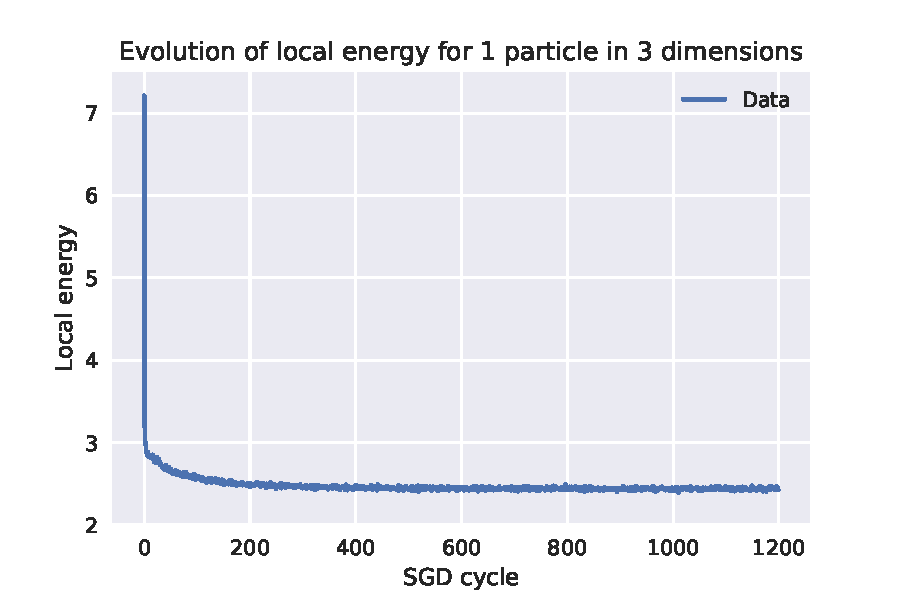
\includegraphics[width=\textwidth]{plot_final1_2.pdf}
%		\caption{}
%	\end{subfigure}
		\centering
		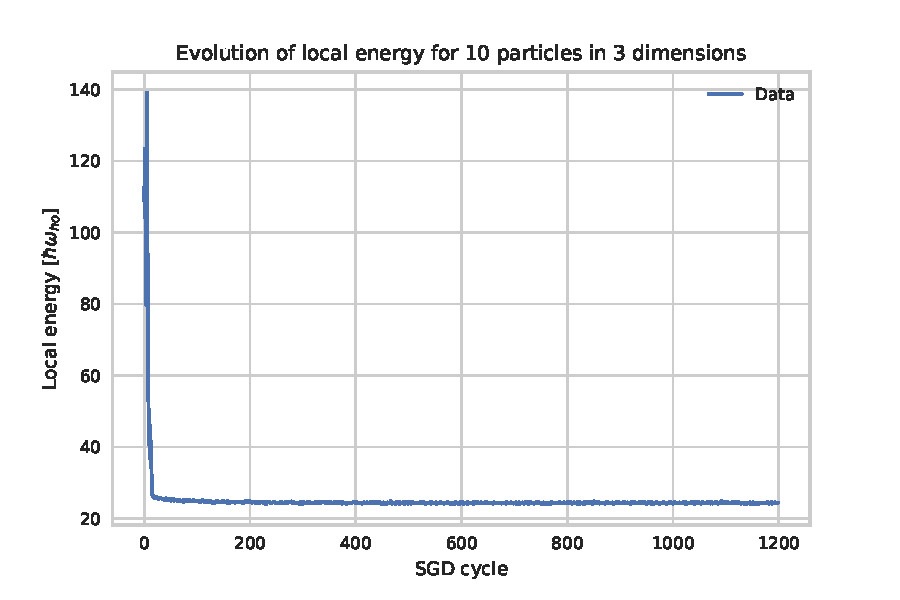
\includegraphics[scale=1.0]{plot_final10.pdf}
	\caption{In this figures, we plot the evolution of ten particles in three dimensions as the program adapts with SGD. We use M $=8$ and $\eta=0.01$. As we can see the local energy converges quickly.}
	\label{Fig:7_8}
\end{figure}

We plot in Fig. (\ref{Fig:7_8}) the results of the first configuration carried out with a $\sigma$ (which gives the spread of the initial parameters according to a Gaussian distribution) of $0.1$ to prove that the RBM is effectively learning. Nevertheless, we note that after $N_p=10$ we need to increase M since the number of particles increases. This process requires to decrease the learning rate to keep stability. By consequence the program becomes much slower to converge to a value: the increment of computational time is dramatic. Therefore, we decide to decrease $\sigma$ to the value of $0.01$. With this choice, we can save some SGD cycle since we have already proven the learning of the RBM. Since we need a much greater number of SGD cycles to find equilibrium with respect to the non-interacting case, we select a number of 1200 SGD cycles. To save time we select $10^5$ MC steps. In the following table we summarize our choices of $N_p$, D, M and we show the results obtained: 


\begin{table}[H]
	\centering
	\caption{Setup used with the various configurations and results obtained: we show the number of hidden nodes $M$, learning rate $\eta$, acceptance rate for each configuration. The learning rate remains constant as we increase the number of particles whereas M is increased each time. The learning rate $\eta$ is the same for $N_p\geq20$. }
	\begin{tabular}{c c |c c c | c} 
		$\boldsymbol{N_p}$ & \textbf{D}  & \textbf{M} & $\boldsymbol{\eta}$ & \textbf{Acceptance rate} &\textbf{Results}\\  
		&&&&&$[\hbar\omega_{ho}]$\\\hline
		10 & 3 & 8 & 0.01  & 0.89 & $\SI{2.44\pm 0.01}{}$ \\
		20 & 3 & 25 & 0.001 & 0.89 & $\SI{2.47\pm 0.01}{}$\\
		30 & 3 & 27 & 0.001 & 0.89 & $\SI{2.47\pm 0.01}{}$\\
		40 & 3 & 30 & 0.001 & 0.89 & $\SI{2.48\pm 0.01}{}$\\
		50 & 3 & 40 & 0.001 & 0.88 & $\SI{2.50 \pm 0.01}{}$\\ 
		60 & 3 & 52 & 0.001 &      &                \\
		70 & 3 & 54 & 0.001 &      &                \\
		80 & 3 & 56 & 0.001 &   0.89   &  $\SI{2.56\pm0.01}{}$              \\
		90 & 3 & 58 & 0.001 &      &                \\
		100 & 3 & 60 &  0.001   &  0.89     &    $\SI{2.63\pm 0.02}{}$           \\
	\end{tabular}
	\label{Tab:4}
\end{table} 

For each configuration, after having checked approximately where the system equilibrates, we take all the mean energies after that point and we take the mean of all of those propagating the uncertainties obtained with the blocking method. The results are shown in Tab. \ref{Tab:4}. 
Furthermore we consider the results obtained from the GP equation in \cite{DalfString} and we check that ours follow the same trend in the small number of particle regime. In Fig. (\ref{Fig:9}), we show how our ML results (blue points) behave in the range $[0,100]$ and $[0,500]$ with respect to GP (red points). The uncertainties are really small, it is not possible to see them from the figure. We plot also the energy per particle with $N_p=1$ (green triangle) which is still a non-interacting case, just as a guide for the reader to follow the GP trend below $N_p=100$. As we can see the energy per particle increases as we increase the number of particles coherently with GP. However, the ML data seem to underestimate the GP trend. This problem could mean that we have not used enough hidden nodes. Nevertheless it should be noted that with $N_p=100$, the maximum number of hidden nodes possible is found to be M $=60$. If we increase M above this value, either the energy diverges immediately or we obtain negative energies. This configuration corresponds to $18360$ variational parameters. This seems to be our limit.\\
The error is quite constant as we increase $N_p$, it grows for $N_p=100$. This is due to the fact that the increment of $N_p$, M makes the system less able to stabilize around a value (the fluctuations become bigger and bigger). In order to decrease the error, we should increase the number of Monte Carlo step, this has not been done here since it would have been computationally too expensive.\\
As regards $E_L/N_p$ for $N_p=100$, in \cite{DalfString} the result of $2.66\ \hbar\omega_{ho}$ is reported. We obtain $\SI{2.63\pm 0.02}{}\ \hbar\omega_{ho}$ which agrees within $2\sigma$ with the GP result. 

\begin{figure}[H]
	\centering
	\centerline{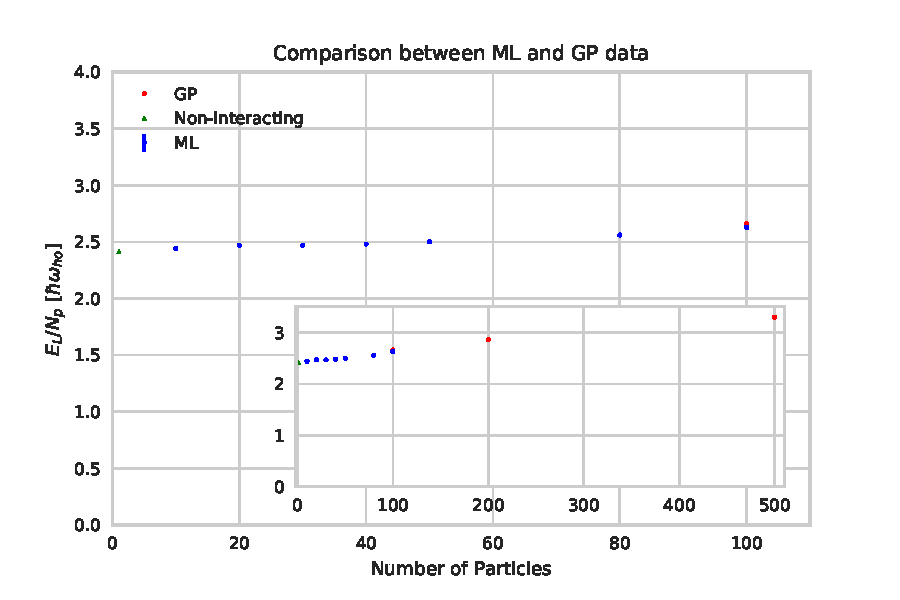
\includegraphics[scale=1.2]{plot_finale.pdf}}
	\caption{Comparison between ML data from our code (blue dots) and the GP results (red dots) in \cite{DalfString} in the range $[0,100]$ and $[0,500]$. The green triangle is the expected $E_L/N_p$ for $N_p=1$: in this situation we are still in the non-interacting case. The point is inserted to help the reader to follow the GP trend below $N_p=100$. ML data seem to underestimate the GP results. This problem is probably related to the insufficient number of hidden nodes used.}
	\label{Fig:9}
\end{figure} 
	\end{chapter}
\end{part}
 
% PART IV: CONCLUSIONS
\begin{part}{Conclusions}
	\label{part:conclusion}
	\begin{chapter}{Summary and Outlook}
		\label{chap:conclusion}
		We started this work with two main goals: the first was to verify whether it was possible to apply Machine Learning methods to compute the ground state energy of a BEC and secondly whether it was possible to learn something more about the Restricted Boltzmann Machine itself. We can safely state that we were able to accomplish both goals. 

We were able to write an object-oriented code in C++ which computes the energy of a Bose-Einstein condensate through Variational Monte Carlo methods with a trial wave-function constructed with the RBM. The algorithms used to compute energy, errors and to sample were discussed. The Importance Sampling Metropolis-Hastings algorithm was found to produce smaller errors than the Brute Force Metropolis one. The code was benchmarked with the case of non-interacting particles in a spherical harmonic potential with satisfactory results. On the other hand, the test with non-interacting particles in an elliptical harmonic potential was a failure. We were able to fix this problem by biasing the z direction with ad hoc parameters found through a trial and error procedure. Nevertheless, we have discovered that the Restricted Boltzmann Machine faces serious problems when it has to a learn an elliptical symmetry. \\
As regards interacting particles in an elliptical harmonic potential, we computed the local energy per particle $E_L/N_p$ for $N_p=10,20,30,40,50,60,70,80,90,100$. We compared the results with the ones obtained from GP equation (eq. (\ref{GP})) in \cite{DalfString}. Even though the trend was similar to GP, our results seemed to underestimate GP for $N_p>20$. We argue that our algorithms might be affected by a systematic error that we are not able to evaluate with our statistical analysis. Therefore, further analysis are needed. Nevertheless, we note that this problem could be fixed by increasing the number of hidden nodes at the cost of increasing abruptly the computational time. Anyway, we should take into account that that our limit with this current setup is about N $=300$ visible nodes and M $=60$ invisible nodes. As we noted this leads to 18360 total parameters to adjust at each interaction. \\
We report the result with $N_p=100$:
\begin{equation*}
	\frac{E_L}{N_p}=\SI{2.63\pm 0.02}{}\ \hbar\omega_{ho}
\end{equation*} 
which can be directly compared with $E_L/N_p=2.66\  \hbar\omega_{ho}$ obtained from GP in \cite{DalfString}. The agreement is really good.

In \cite{carleoSolvingQuantumManybody2017} Carleo and Troviks were able to apply ML to a chain of $80$ spins and a $10\times 10$ lattice. Therefore, having been able to apply ML to $100$ interacting particles in an elliptical harmonic potential in 3D can be considered a satisfactory result.  


Nevertheless, the are several improvements that we can implement in our code. First of all, we can find a way to parallelize it in order to gather more data and to lower the error. \\
Instead of fixing the elliptical symmetry with two ad hoc parameters such as $\xi_1$ and $\xi_2$, we could insert two variational parameters in those positions initialized with the values of $\xi_1$ and $\xi_2$ which we have found. In this way, the RBM should be able to represent the elliptical symmetry with more precision. \\
Another interesting test would be to modify RBM or to implement some other machine in order to check whether we are able to increase the number of particles as well as the number of hidden nodes without breaking the stability. \\
Overall we should speed up the code. This would allow us to increase the number of SGD cycles and, in particular, of hidden nodes without increasing dramatically the computational time.\\
Other limitations regard the Stochastic Gradient Descent method such as the oscillation of the energy in the elliptical case and the constraint to set a fixed learning rate. In particular, the second led to divergent energy if $\eta$ had been set too high, or slow convergence if it had been set too small. Therefore, firstly, we should update our algorithm by adding the so-called Momentum method which accelerates the SGD in the relevant direction. As a consequence it lowers the oscillations. This is straightforward to implement. Then, we should introduce a dynamic learning rate which adapts itself at each cycle. Examples are countless: RMSProp (Root Mean Square Propagator), Adam (Adaptive Moment Estimation), ADAdelta, etc. They are all quite similar. Hence the task would be to understand which one is the best for our case and then to implement it. 




	\end{chapter}	
	% \begin{chapter}{Future Developements}
	% 	\label{chap:future}
	% 	\input{conclusion/future}
	% \end{chapter}
\end{part}

\cleardoublepage


% APPENDICES



\begin{appendices}
	
	\begin{part}{Appendix}
	\end{part}
\end{appendices}
	
% MAKE BIBLIOGRAPHY
%\bibliographystyle{unsrt}
%bibliography/master_thesis_1}
\printbibliography

 
 
% AND SO WE END
\end{document}
